\documentclass[11pt,xcolor=pdftex,dvipsnames,table,t]{beamer}
%adding handout above here kills pause
\usefonttheme[onlymath]{serif}
%\usetheme{default}
\usetheme{Hannover}
%\usepackage{times}
%\usefonttheme{structurebold}

\usepackage[english]{babel}
%\usepackage[table]{xcolor}
\usepackage{amsmath}
\usepackage{pgf,pgfarrows,pgfnodes,pgfautomata,pgfheaps}
\usepackage{amsmath,amssymb,setspace}
\usepackage[latin1]{inputenc}
\usepackage[T1]{fontenc}
\usepackage{relsize}
\usepackage{comment}

%RICH NOTE: this was causing errors for me
%\usepackage{pxfonts}

\usepackage[absolute,overlay]{textpos} 
\newenvironment{reference}[2]{% 
  \begin{textblock*}{\textwidth}(#1,#2) 
      \footnotesize\it\bgroup\color{red!50!black}}{\egroup\end{textblock*}} 

\DeclareMathSizes{10}{10}{6}{6} 

%rich added 
\setbeamertemplate{navigation symbols}{}
\setbeamertemplate{footline}[frame number]

\addtobeamertemplate{frametitle}{\vspace*{-.20cm}}{\vspace*{0.1cm}}

\usepackage{hyperref}
% Change the setup later on, after loading hyperref
\hypersetup{colorlinks=true, urlcolor=blue, linkcolor=blue, citecolor=blue, linktocpage}

% Bib stuff

\usepackage{natbib}
\usepackage{bibentry}
%\renewcommand{\cite}{\citet}
%\let\oldcite=\cite                                                          %\renewcommand{\cite}[1]{\textcolor[rgb]{0,0,1}{\oldcite{#1}}}
%\renewcommand{\cite}{\citet}



\title{Treatment Effects}
\author{Charlie Murry and Richard L. Sweeney}
\institute{based on slides by Chris Conlon}
\date{Empirical Methods \\ Spring 2019}

\setbeamerfont{equation}{size=\tiny}
\DeclareMathSizes{10}{10}{6}{6} 

\begin{document}

\begin{frame}
    \titlepage
\end{frame}

\begin{frame}
    \tableofcontents  
\end{frame}

\frame{\frametitle{Overview}

This lecture draw heavily upon 
\begin{itemize}
\item 2012 AEA continuing education lectures by Imbens and Woodldridge (full materials available \href{https://www.aeaweb.org/webcasts/2012/}{here}.)
\item \citet{AbadieCattaneoAnRev2018}
\end{itemize}

}

\section{Setup}

\begin{frame}
\frametitle{The Evaluation Problem}
\begin{itemize}
\item The issue we are concerned about is identifying the effect of a policy or an investment or some individual action on one or more outcomes of interest
\item This has become the workhorse approach of the applied microeconomics fields (Public, Labor, etc.)
\item Examples may include:
\begin{itemize}
\item The effect of taxes on labor supply
\item The effect of education on wages
\item The effect of incarceration on recidivism
\item The effect of competition between schools on schooling quality
\item The effect of price cap regulation on consumer welfare
\item The effect of indirect taxes on demand
\item The effects of environmental regulation on incomes
\item The effects of labor market regulation and minimum wages on wages and employment
\end{itemize}
\end{itemize}
\end{frame}

\begin{frame}
  \frametitle{Setup}
  Typically attributed to Donald Rubin
  \begin{itemize}
  \item Observe $N$ units, indexed by $i$, drawn randomly from a larger population
  \item Postulate two \alert{potential outcomes} for each unit $\{Y_i(1), Y_i(0)\}$ depending on whether they receive treatment or not.
  \item Observe additional \textit{exogenous} covariates $X_i$
  \item Consider a binary treatment $W_i$ such that 
  \begin{equation*}
    Y_{i} \equiv Y_i(W_i) = 
      \begin{cases}
        Y_i(0) & \text{if $W_i=0$}\\
        Y_i(1) & \text{if $W_i=1$}
      \end{cases}       
  \end{equation*}
\end{itemize}
\end{frame}

\begin{frame}
  \frametitle{SUTVA}
  \begin{itemize}
  \item Note there is already an important assumption embedded in this setup, the stable unit treatment value assumption (\alert{SUTVA}). 
  \item Assume that the outcome, in either state for unit $i$ does not depend on the assignment of other units.   
  \item This is likely to fail in many important settings. 
  \item Two ways to express this:
  \begin{itemize}
  	\item No interference.
  	\item No hidden variations
  \end{itemize}
  \item Examples?
\end{itemize}
\end{frame}

\begin{frame}
  \frametitle{Methods}
  \begin{enumerate}
  \item Matching
  \item Instrumental Variables
  \item Difference in Difference and Natural Experiments
  \item RCTs
  \item Structural Models
  \end{enumerate}
  \begin{itemize}
  \item Key distinction: the treatment effect of some program (a number) from understanding how and why things work (the mechanism).
  \item Models let us link numbers to mechanisms.
  \end{itemize}
\end{frame}

\begin{frame}
  \frametitle{The Evaluation Problem}
  \begin{itemize}
  \item Two major problems:
  \begin{itemize}
  \item All individuals have different treatment effects (\alert{heterogeneity}).
  \item We don't actually observe any one person's treatment effect ! (Missing Data problem)
  \item Individual treatment effects $\tau_i = Y_{1i} - Y_{0i}$ are never observed (FPOCI)
  \end{itemize}
  \item We need strong assumptions in order to recover $f(\beta_i)$ from data.
  \end{itemize}
\end{frame}

\begin{frame}
  \frametitle{More Difficulties}
  What is hard here?
  \begin{itemize}
  \item Heterogeneous effect of $\beta_i$ in population.
  \item Selection in treatment may be endogenous. That is $W_i$ depends on $Y_i(1),Y_i(0)$.
  \item Fisher or Roy (1951) model:
  \begin{eqnarray*}
  Y_i = (Y_i(1) - Y_i(0)) W_i + Y_i(0)= \alpha + \beta_i W_i + u_i
  \end{eqnarray*}
  \item Agents usually choose $W_i$ with $\beta_i$ or $u_i$ in mind.
  \item Can't necessarily pool across individuals since $\beta_i$ is not constant.
  \end{itemize}
\end{frame}


\begin{frame}
  \frametitle{Structural vs. Reduced Form}
  \begin{itemize}
  \item Usually we are interested in one or two parameters of the distribution of $\beta_i$ (such as the average treatment effect or average treatment on the treated).
  \item Most program evaluation approaches seek to identify one effect or the other effect. This leads to these as being described as \alert{reduced form} or \alert{quasi-experimental}.
  \item The \alert{structural} approach attempts to recover the entire joint $f(\beta_i,u_i)$ distribution but generally requires more assumptions, but then we can calculate whatever we need.
  \item Instead we often focus on simpler estimands.
  \end{itemize}
\end{frame}

\begin{frame}
  \frametitle{Common Objects of Interest}
  \begin{itemize}
    \item Population average treatment effect (PATE)
      $$ \tau_P = E \left[ Y_i(1) - Y_i(0) \right] $$
    \item Population average treatment effect for treated units (PATT)
      $$ \tau_{P,T} = E \left[ Y_i(1) - Y_i(0) | W = 1 \right] $$
    \item Sample average treatment effect (SATE)
      $$ \tau_S = \frac{1}{N} \sum_{i=1}^N ( Y_i(1) - Y_i(0) ) $$
    \item Sample average treatment effect for treated units (SATT)
      $$ \tau_{S,T} = \frac{1}{N_T} \sum_{i \in W_i=1} ( Y_i(1) - Y_i(0) ) $$
  \end{itemize}
\end{frame}

\subsection{Conditional Independence}

%TK add abadia DAG here. 
\begin{frame}
  \frametitle{Confounding}
  \begin{itemize}
  \item Consider the \textit{association} 
  $$ \tau = E \left[ Y | W= 1 \right] - E \left[ Y | W= 0 \right] $$
  \item Then $ \tau = \tau_{ATE} + b_{ATE} $
  \item Where $b$ is the \textit{bias}
  \begin{multline*}
    b_{ATE} =  ( E \left[ Y_1 | W= 1 \right] - E \left[ Y_1 | W= 0 \right])Pr(W=0) \\ 
              + ( E \left[ Y_0 | W= 1 \right] - E \left[ Y_0 | W= 1 \right])Pr(W=1) 
  \end{multline*}
  \item So the bias disapears only if the potential outcomes are independent of treatment assignment. 
  \item This is called \textbf{unconfoundedness}. 
  \end{itemize}
\end{frame}
  
\begin{frame}
  \frametitle{Estimation under unconfoundedness}
   \textbf{Assumption: 1 } $$ \left(Y_i(0),Y_i(1) \right) \perp W_i | X_i $$
  \begin{itemize}
  \item Sometimes called ``conditional independence assumption'' or ``selection on observables''. 
  \item Can see this is implicit in the regression $Y_i = \alpha + \tau W_i + X_i'\beta + \epsilon_i$ where $\epsilon_i \perp X_i$ 
  under the assumption of a constant treatment effect (otherwise this is not the same)
  \end{itemize}

  \textbf{Assumption 2  (Overlap)} $$ 0 < Pr(W_i = 1 | X_i) < 1 $$
\end{frame}
  
\begin{frame}
  \frametitle{How useful are these assumptions?}
  \citet{imbens2015matching} has a good discussion on this. Suggests following motivations: 
  \begin{itemize}
    \item This is a natural starting point. Compare treatment and control units, after adjusting for observables. Need not be the last word! 
    \item \textit{All} comparisons involve comparing treated to untreated units. Absent RCT, its up to researcher to investigate which comparisons to emphasize
    \item Often specifying a model can clarify how sensible this is. Guido has a good example on costs in the paper. 
  \end{itemize} 
\end{frame}

\begin{frame}
  \frametitle{Under these assumptions, can we just use regression?}
  \begin{itemize}
    \item Let $\mu_w(x) = E [Y_i(w) | X_i = x] $
    \item A regression estimate of $\tau$ is then 
     $$ \hat \tau_{reg} = \frac{1}{N} \sum_i W_i(Y_i - \hat \mu_0(X_i)) + (1-W_i)(\hat \mu_1(X_i) -  Y_i ) $$
    \item Typically estimate $$ Y_i = \alpha  + \beta'X_i + \tau W_i + \epsilon_i $$ which assumes $\mu_w(x) = \beta' x + \tau*w $ 
    \item Could easily also compute $$\mu_w(x) = \alpha_w + \beta_w'x$$
    \item Key point is that this estimator can be viewed as a \alert{missing data} problem, where predictions are computed using regression. 
  \end{itemize} 
\end{frame}

\begin{frame}
  \frametitle{When is this likely to be a problem?}
  \begin{itemize}
    \item Note $\mu_0(x)$ is used to predict the "missing" control outcomes for the treated observations.
    \item Want this predition at the average treated covariates $\bar X_T$
    \item With linear regression, our average control prediction for the treated observations is going to be $\bar Y_C + \hat \beta'(\bar X_T - \bar X_C)$ 
    \item Ok if: 
    \begin{enumerate}
      \item $\mu()$ is properly specified
      \item treated and control observations are similar (in $X$)
    \end{enumerate}
    \item First condition is untestable, but in practice predictions are often sensitive to functional form
    \item Leads to a big emphasis on covariate balance. 
  \end{itemize} 
\end{frame}

\section{Matching}

\begin{frame}
\frametitle{Matching}
\begin{itemize}
\item Regression imputes missing potential outcomes using regression. 
\item Matching imputes using the \textit{realized} outcome of (nearly) identical units in the opposite assignment group. 
\item Remember, we're in a world where we've assumed unconfoundedness. Only challenge is that the treatment group and the control group don't have the same distribution of $X$'s. 
\item \alert{Re-weight} the un-treated population so that it resembles the treated population.
\item Once distribution of $X_i$ is the same for both groups $ X_i | W_i \sim X_i$ then we assume all other differences are irrelevant and can just compare means.
\end{itemize}
\end{frame}

\begin{frame}
\frametitle{Matching}
Let  $F^{1}(x)$ be the distribution of characteristics in the treatment group, we can define the ATE as 
\begin{eqnarray*}
&&E[Y(1) - Y(0) | T =1] = E_{F^1(x)} [E(Y(1) -Y(0) | T=1,X)] \\
&=&  E_{F^1(x)} [E(Y(1) | T=1,X)] -  E_{F^1(x)} [E(Y(0) | T=1,X)] \mbox{ linearity } 
\end{eqnarray*}
The first part we observe directly:
\begin{eqnarray*}
&=&  E_{F^1(x)} [E(Y(1) | T=1,X)] 
\end{eqnarray*}
But the counterfactual mean is not observed!
\begin{eqnarray*}
&=&  E_{F^1(x)} [E(Y(0) | T=1,X)] 
\end{eqnarray*}
But conditional independence does this for us:
\begin{eqnarray*}
 E_{F^1(x)} [E(Y(0) | T=1,X)]  =  E_{F^1(x)} [E(Y(0) | T=0,X)] 
\end{eqnarray*}
\end{frame}

\begin{frame}
\frametitle{A Matching Example}
Here is an example where matching was helpful from a paper by Prof. Mortimer:
\begin{itemize}
\item She ran a randomized experiment where we removed Snickers bars from around 60 vending machines in office buildings in downtown Chicago.
\item There are a few possible control groups:
\begin{enumerate}
\item Same vending machine in other weeks (captures heterogeneous tastes in the cross section)
\item Other vending machines in the same week (might capture aggregate shocks, ad campaigns, etc.)
\end{enumerate}
\item We went with \#1 as \#2 was not particularly helpful.
\end{itemize}
\end{frame}

\begin{frame}
\frametitle{A Matching Example}
Major problem was that there was a ton of heterogeneity in the overall level of (potential) weekly sales which we call $M_t$.
\begin{itemize}
\item Main source of heterogeneity is how many people are in the office that week, or how late they work.
\item Based on total sales our average over treatment weeks was in the 74th percentile of all weeks.
\item This was after removing a product, so we know sales should have gone down!
\item How do we fix this without running the experiment for an entire year!
%\item Can't use shares instead of quantities. Why?
\end{itemize}
\end{frame}

\begin{frame}
\begin{center}
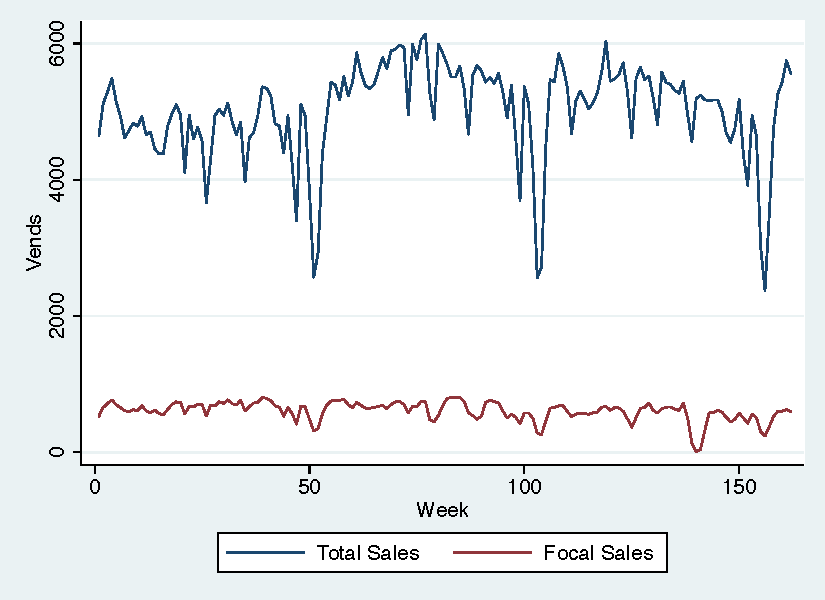
\includegraphics[width=4in]{./resources/figure1.pdf}
\end{center}
\end{frame}

\begin{frame}
\frametitle{A Matching Example}
Ideally we could just observe $M_t$ directly and use that as our matching variable $X$
\begin{itemize}
\item We didn't observe it directly and tried a few different measures:
\begin{itemize}
\item Sales at the soda machine next to the snack machine
\item Sales of salty snacks at the same machine (not substitutes for candy bars).
\item We used k-NN with $k=4$ to select control weeks -- notice we re-weight so that overall sales are approximately same (minus the removed product).
\end{itemize}
\item We also tried a more structured approach:
\begin{itemize}
\item Define controls weeks as valid IFF
\item Overall sales were weakly lower
\item Overall sales were not less than Overall Sales less expected sales less Snickers Sales.
\end{itemize}
\end{itemize}
\end{frame}


\begin{frame}
\begin{table}
\begin{center}
\tiny
\label{tab:nonparam}
\begin{tabular}{|l|rrrcrrcr|}
\hline
 & Control  & Control & Treatment& \hspace{-0.3in}& Treatment & Mean & \hspace{-0.3in} & \\
Product & Mean &  \%ile & Mean& \hspace{-0.3in} & \%ile &  Difference & \hspace{-0.3in}& \% $\Delta$\\
\hline \hline
\multicolumn{9}{|l|}{\emph{Vends}} \\ \hline
Peanut M\&Ms&359.9&73.6&478.3&\hspace{-0.3in}*&99.4&118.4& \hspace{-0.3in}*&32.9\\
Twix Caramel&187.6&55.3&297.1&\hspace{-0.3in}*&100.0&109.5& \hspace{-0.3in}*&58.4\\
Assorted Chocolate&334.8&66.7&398.0&\hspace{-0.3in}*&95.0&63.2& \hspace{-0.3in}*&18.9\\
Assorted Energy&571.9&63.5&616.2& \hspace{-0.3in}&76.7&44.3 & \hspace{-0.3in} &7.8\\
Zoo Animal Cracker&209.1&78.6&243.7&\hspace{-0.3in}*&98.1&34.6& \hspace{-0.3in}*&16.5\\
Salted Peanuts&187.9&70.4&216.3&\hspace{-0.3in}*&93.7&28.4 & \hspace{-0.3in} &15.1\\
Choc Chip Famous Amos&171.6&71.7&193.1&\hspace{-0.3in}*&95.0&21.5& \hspace{-0.3in}*&12.5\\
Ruger Vanilla Wafer&107.3&59.7&127.9& \hspace{-0.3in}&78.6&20.6& \hspace{-0.3in}*&19.1\\
Assorted Candy&215.8&43.4&229.6& \hspace{-0.3in}&60.4&13.7& \hspace{-0.3in}&6.4\\
Assorted Potato Chips&279.6&64.2&292.4&\hspace{-0.3in}*&66.7&12.8& \hspace{-0.3in}&4.6\\
Assorted Pretzels&548.3&87.4&557.7&\hspace{-0.3in}*&88.7&9.4& \hspace{-0.3in}&1.7\\
Raisinets&133.3&66.0&139.4& \hspace{-0.3in}&74.2&6.1& \hspace{-0.3in}&4.6\\
Cheetos&262.2&60.1&260.5& \hspace{-0.3in}&58.2&-1.8& \hspace{-0.3in}&-0.7\\
Grandmas Choc Chip&77.9&51.3&72.5& \hspace{-0.3in}&37.8&-5.4& \hspace{-0.3in}&-7.0\\
Doritos&215.4&54.1&203.1& \hspace{-0.3in}&39.6&-12.3& \hspace{-0.3in}*&-5.7\\
Assorted Cookie&180.3&61.0&162.4& \hspace{-0.3in}&48.4&-17.9& \hspace{-0.3in}&-10.0\\
Skittles&100.1&62.9&75.1&\hspace{-0.3in}*&30.2&-25.1& \hspace{-0.3in}*&-25.0\\
Assorted Salty Snack&1382.8&56.0&1276.2&\hspace{-0.3in}*&23.3&-106.7& \hspace{-0.3in}*&-7.7\\
Snickers&323.4&50.3&2.0&\hspace{-0.3in}*&1.3&-321.4& \hspace{-0.3in}*&-99.4\\ \hline
Total&5849.6&74.2&5841.3& \hspace{-0.3in}&73.0&-8.3& \hspace{-0.3in}&-0.1\\
\hline\end{tabular}
\end{center}
\tiny
Notes: Control weeks are selected through the-neighbor matching using four control observations for each treatment week.  Percentiles are relative to the full distribution of control weeks.
\end{table}
\end{frame}


\begin{frame}
\frametitle{How do you actually do this?}  
\begin{itemize}
  \item One dimension is easy: just sort 
  \item In multiple dimensions, there are a variety of built in nearest neighbor packages (Abadie Imbens (2006))
  \item What's nice about these is that the reasearcher only has to pick the number of matches (although the default tolerances not always innocuous)
  \item This is still cursed in that our nearest neighbors get further away as the dimension grows.
  \item Suppose instead we had a \alert{sufficient statistic}
\end{itemize}
\end{frame}

\begin{frame}
\frametitle{Propensity Score}
\begin{itemize}
\item Rosenbaum and Rubin propose the \alert{propensity score}
\begin{eqnarray*}
e(x) = Pr(W_i  = 1 | X_i) = E[W_i | X_i = x]
\end{eqnarray*}
\item They prove that under the assumption of unconfoundedness, 
  $$ (Y_i(0),Y_i(1)) \perp W_i | e(X_i) $$ 
\item So even if $X$ is high dimensional, it is sufficient to condition on a scalar function 
\item Of course, the true propensity score is not known... 
\end{itemize}
\end{frame}

\begin{frame}
  \frametitle{This suggests an attractive weigthing}
  \begin{center}
    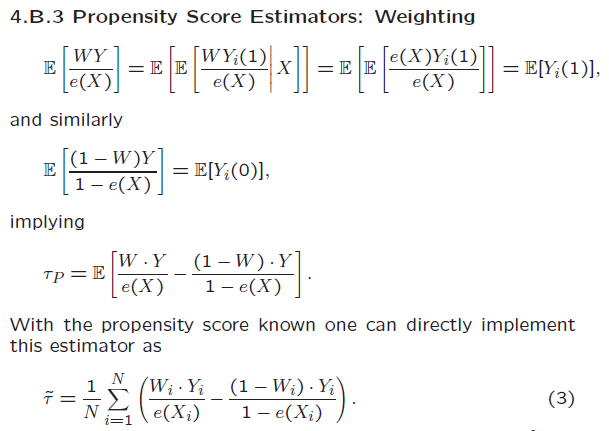
\includegraphics[scale=0.55]{./resources/imbensAEAPsWeight}
  \end{center}  
\end{frame}

\begin{frame}
  \frametitle{Approaches now look similar}
  \begin{itemize}
  \item One option is "inverse probability weighting" 
  \item Nonparametrically estimate $e(x)$, the compute 
  $$ \hat \tau = \sum_i^N \frac{W_i Y_i}{\hat e(X_i)} / \sum_i^N \frac{W_i}{\hat e(X_i)} - \sum_i^N \frac{(1-W_i) Y_i}{1 - \hat e(X_i)} / \sum_i^N \frac{(1-W_i)}{1 - \hat e(X_i)} $$ 
  where this is slightly more complicated than just plugging in $\hat e()$ because in your sample the weights won't necessarily sum to one (Hirano, Imbens and Ridder (2003))
  \item Alternatively we could flexibly estimate $\mu_w$ then plug in these predictions for each observation manually. 
  \item With discrete covariates, these will be equivalent! 
  \item Otherwise there finite sample propoerties will vary depending on the smoothness of the regression and propensity score functions. 
  \end{itemize}
\end{frame}

\begin{frame}
  \frametitle{What about matching on the (estimated) propensity score?}
  \begin{itemize}
  \item VERY widely used approach 
  \item Large sample properties not known 
  \item "Why Propensity Scores Should Not Be Used for Matching" \citep{KingNielsonPSM}
  \item Show this performs poorly in simulations compared to matching on X's directly. 
  \item One alternative from the same author's: Coarsened Exact Matching
  \begin{itemize}
    \item Available in R and Stata from \href{https://gking.harvard.edu/cem}{Gary King's website}
    \item The idea: temporarily coarsen each variable into substantively meaningful groups, exact match on these coarsened data, and then retain only the original (uncoarsened) values of the matched data.
  \end{itemize}
  \end{itemize}
\end{frame}
  
\begin{frame}
  \frametitle{CEM has many uses}
  \begin{itemize}
  \item Linh To's JMP: 
  \item Question: Is there a signal value to parental leave? 
  \item Theory: many PBNE's. In practice depends on pooling. 
  \item Setting: Extension of leave in Denmark. 
  \item Look for response among three types of women: 
  \begin{enumerate}
    \item pool, pool
    \item pool, separate
    \item separate, separate
  \end{enumerate}
  \item Convincing RD: restrict to sample already pregnant when law announced 
  \item Challenge: Only see mothers in one group or the other
  \item Solution: Match each pre period mother using their closest post-period counterpart, and assign her to that post-group. 
  \end{itemize}
\end{frame}

\begin{frame}
  \frametitle{Results}
  \begin{center}
    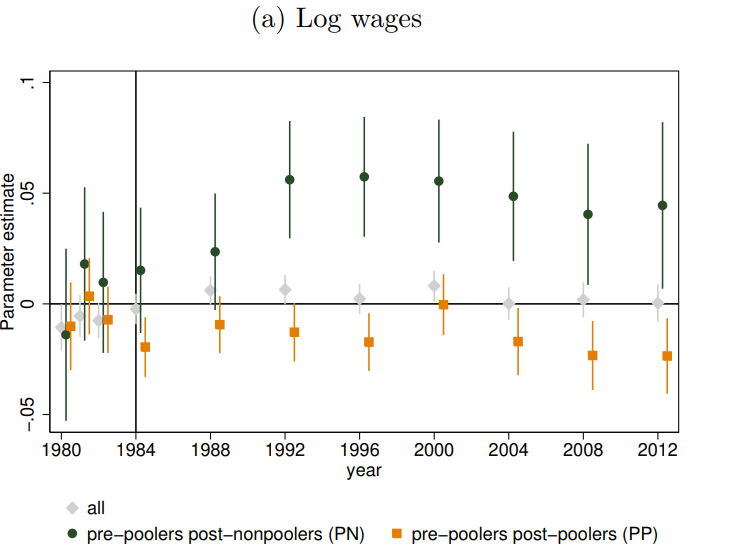
\includegraphics[width=.9\textwidth]{./resources/ToPooling}
  \end{center}  
\end{frame}

%TK Copy susan's jep suggested readings here. 
\begin{frame}
  \frametitle{What can ML add here?}
  \begin{itemize}
  \item Estimating the propensity score is a pure \textbf{prediction} problem. We don't care what causes someone to be treated in this setup
  \item This is a natural place for ML (decision trees, random forests). 
  \item What should we use to predict? 
  \end{itemize}
\end{frame}

\begin{frame}[allowframebreaks]
  \frametitle{Some recent ML proposals}
  Belloni, Chernozhukov, Fernández, and Hansen (2013) \nocite{belloni2015program}
  \begin{itemize}
    \item "double selection" procedure
    \item use LASSO to select $X$ which predict $Y$, and another LASSO to find $X$ that predict $W$ 
    \item then do OLS on the union of the two sets of covariates
    \item show this performs better than simple regularized regression of outcome on treatment and covariates in one step 
  \end{itemize}
  
  \framebreak

  Athey, Imbens, and Wager (2016) \nocite{athey2016efficient} \\
  ``Approximate Residual Balancing: De-Biased Inference of Average Treatment Effects in High Dimensions)''
  \begin{itemize}
    \item Idea: In order to predict the counterfactual outcomes that the treatment
    group would have had in the absence of the treatment, it is necessary to extrapolate from control
    \item This is confounded by imbalance. 
    \item AIW construct weights so these samples are equivalent, and run penalized regression to compute $\tau$ 
  \end{itemize}

\end{frame}

\begin{frame}
\frametitle{Assessing Unconfoundedness}
\begin{itemize}
\item This assumption is fundamentally untestable
\item However people have proposed a number of tests which, if failed, might be \textit{inconsistent} with unconfoundedness. 
\item One option is to look for an "effect" on an untreated group. 
\item Imagine you had one sample of "eligible" units, some who were treated and some who weren't. And another sample of "ineligible" units, all of whom are also untreated by construction. 
\item You could estimate a difference in outcomes within the two untreated groups. If eligible but untreated units look different than uneligible, that should be worrisome. 
\item Imbens lecture does this with the Lalonde data and the CPS. 
\item Another natural approach is to use "psuedo outcomes", like lagged Y. 
\end{itemize}
\end{frame}

\begin{frame}
  \frametitle{Assessing Overlap}
  \begin{itemize}
  \item Obviously want to start with a summary table comparing the means of your treatment and control groups. 
  \item What's a big difference? t-stats reflective of sample size 
  \item Instead report the normalized difference in covariates. According to Imbens, a an average difference bigger than 0.25 standard deviations is worrisome. 
  \item Another alternative is to plot the propensity score for the two groups. 
  \end{itemize}
\end{frame}

\begin{frame}
  \frametitle{Matching wrapup}
  \begin{itemize}
  \item Even under unconfoundedness, very important to ensure overlap
  \item Restrict your sample so that its balanced, using exact matching if low dimensional, coarse or propensity score otherwise
  \item Assess unconfoundedness using a psuedo-outcome if possible 
  \item Run regression on your matched sample 
  \end{itemize}
\end{frame}

\section{IV}
\subsection{Basics}

\begin{frame}
\frametitle{Instrumental Varibales}

See Guido Imben's \href{https://www.nber.org/WNE/slides_5_late7-30-07.pdf}{NBER Slides}.

\end{frame}

\begin{comment}
\begin{frame}
\frametitle{IV Assumptions}
So what does IV do?
\begin{description}
\item [Independence] $Z_i \perp Y_i(1), Y_i(0), T_i(1), T_i(0)$. Instrument is as if randomly assigned and does not directly affect $Y_i$
\item This is not implied by random assignment. In that case there would be four potential outcomes $Y_i(z,t)$
\item [Random Assignment] $Z_i \perp Y_i(0,0), Y_i(0,1), Y_i(1,0), Y_i(1,1), T_i(1), T_i(0)$. 
\item [Exclusion Restriction] $Y_i(z,t) = Y_i(z',t)$ for all $z,z',t$. 
\item Thus we require both RA and ER to guarantee Independence. The second assumption is a substantive one.
\item We only observe $(Z_i,T_i)$ not the pair $T_i(0),T_i(1)$ so we cannot determine compliance types directly! (See the picture)
\end{description}
\end{frame}


\begin{frame}
\frametitle{IV Assumptions}
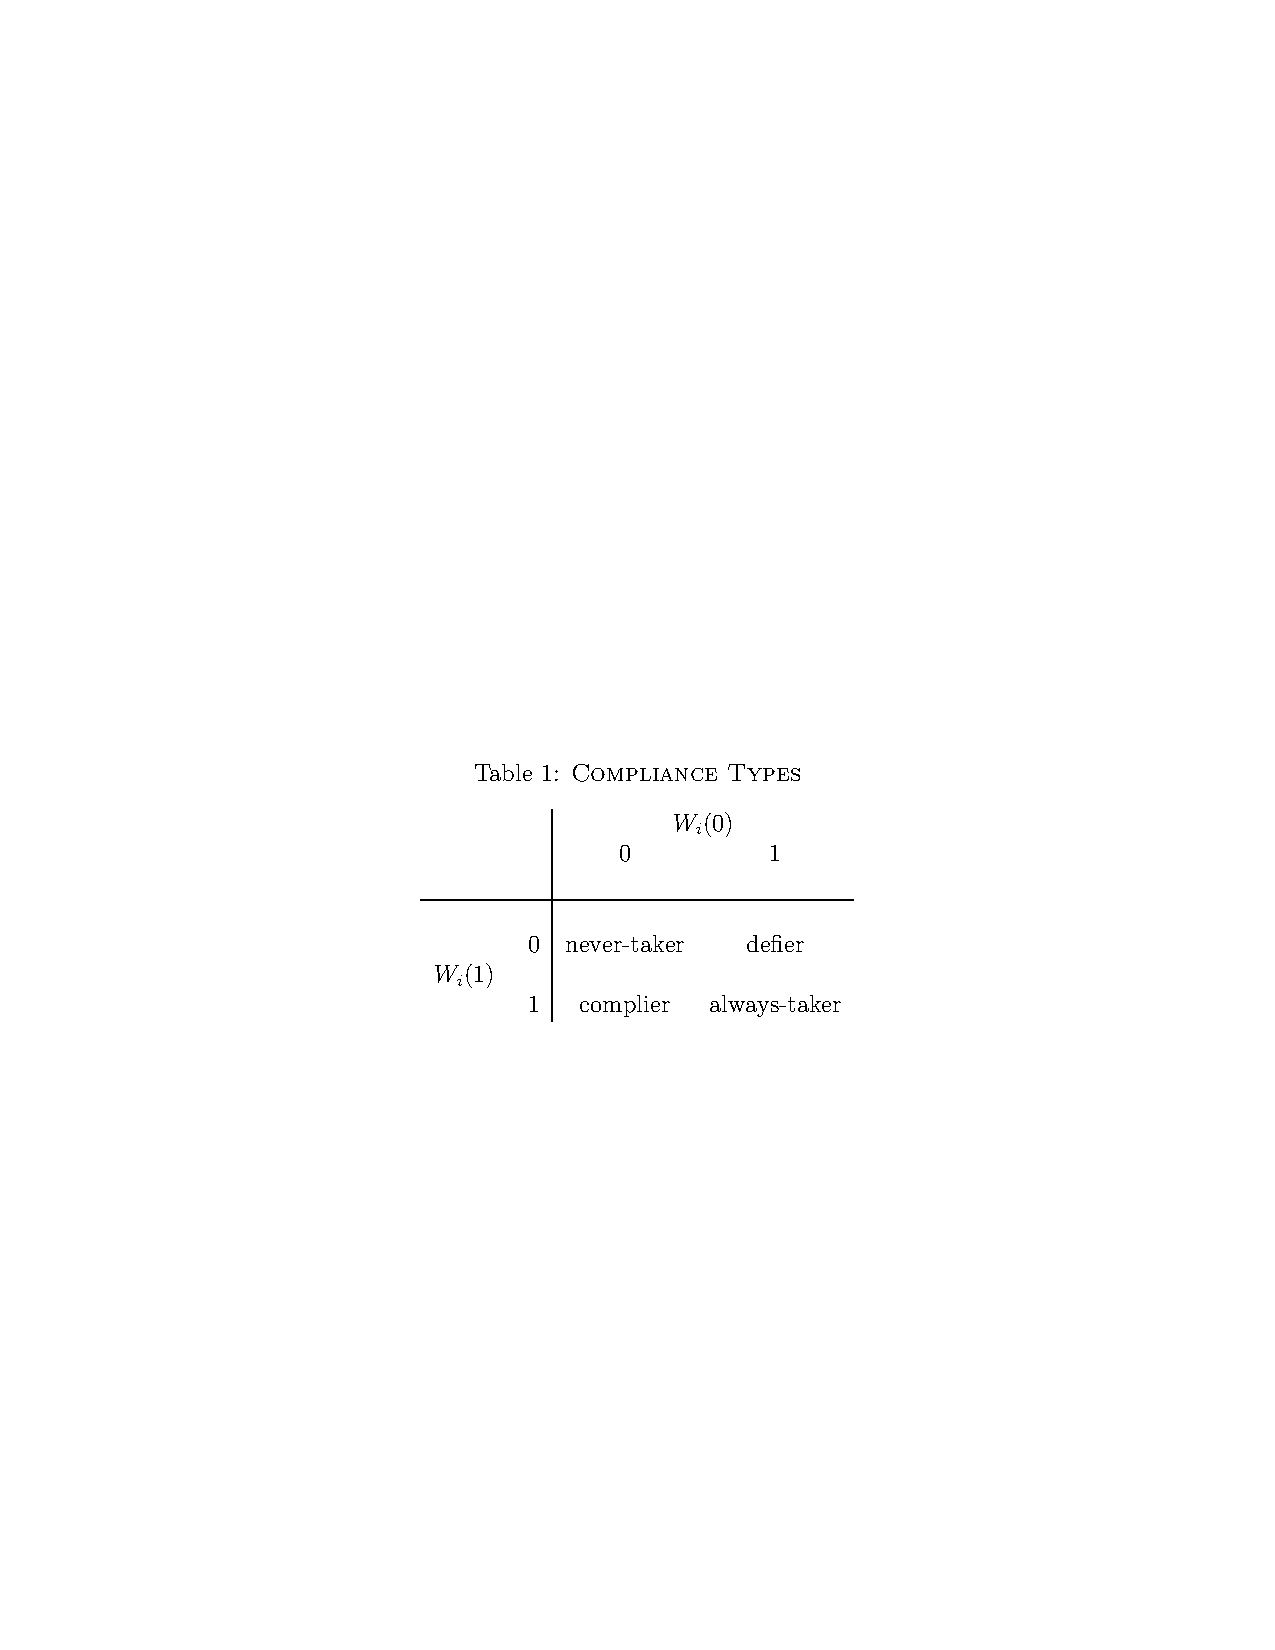
\includegraphics[width=4in]{./resources/imbens1.pdf}
\end{frame}



\begin{frame}
\frametitle{IV Assumptions}
We are stuck without further assumptions, so we assume:
\begin{description}
\item [Monotonicity/No Defiers] $T_i(1) \geq T_i(0)$
\end{description}
\begin{itemize}
\item Works in many applications (classical drug compliance).
\item Implied by many latent index models with constant coefficients
\item Works as long as sign of $\pi_{1,i}$ doesn't change
\begin{eqnarray*}
T_i(z)  = 1 [\pi_0 + \pi_1 z + \varepsilon_i > 0]
\end{eqnarray*}
\end{itemize}
\end{frame}


\begin{frame}
\frametitle{IV Assumptions}
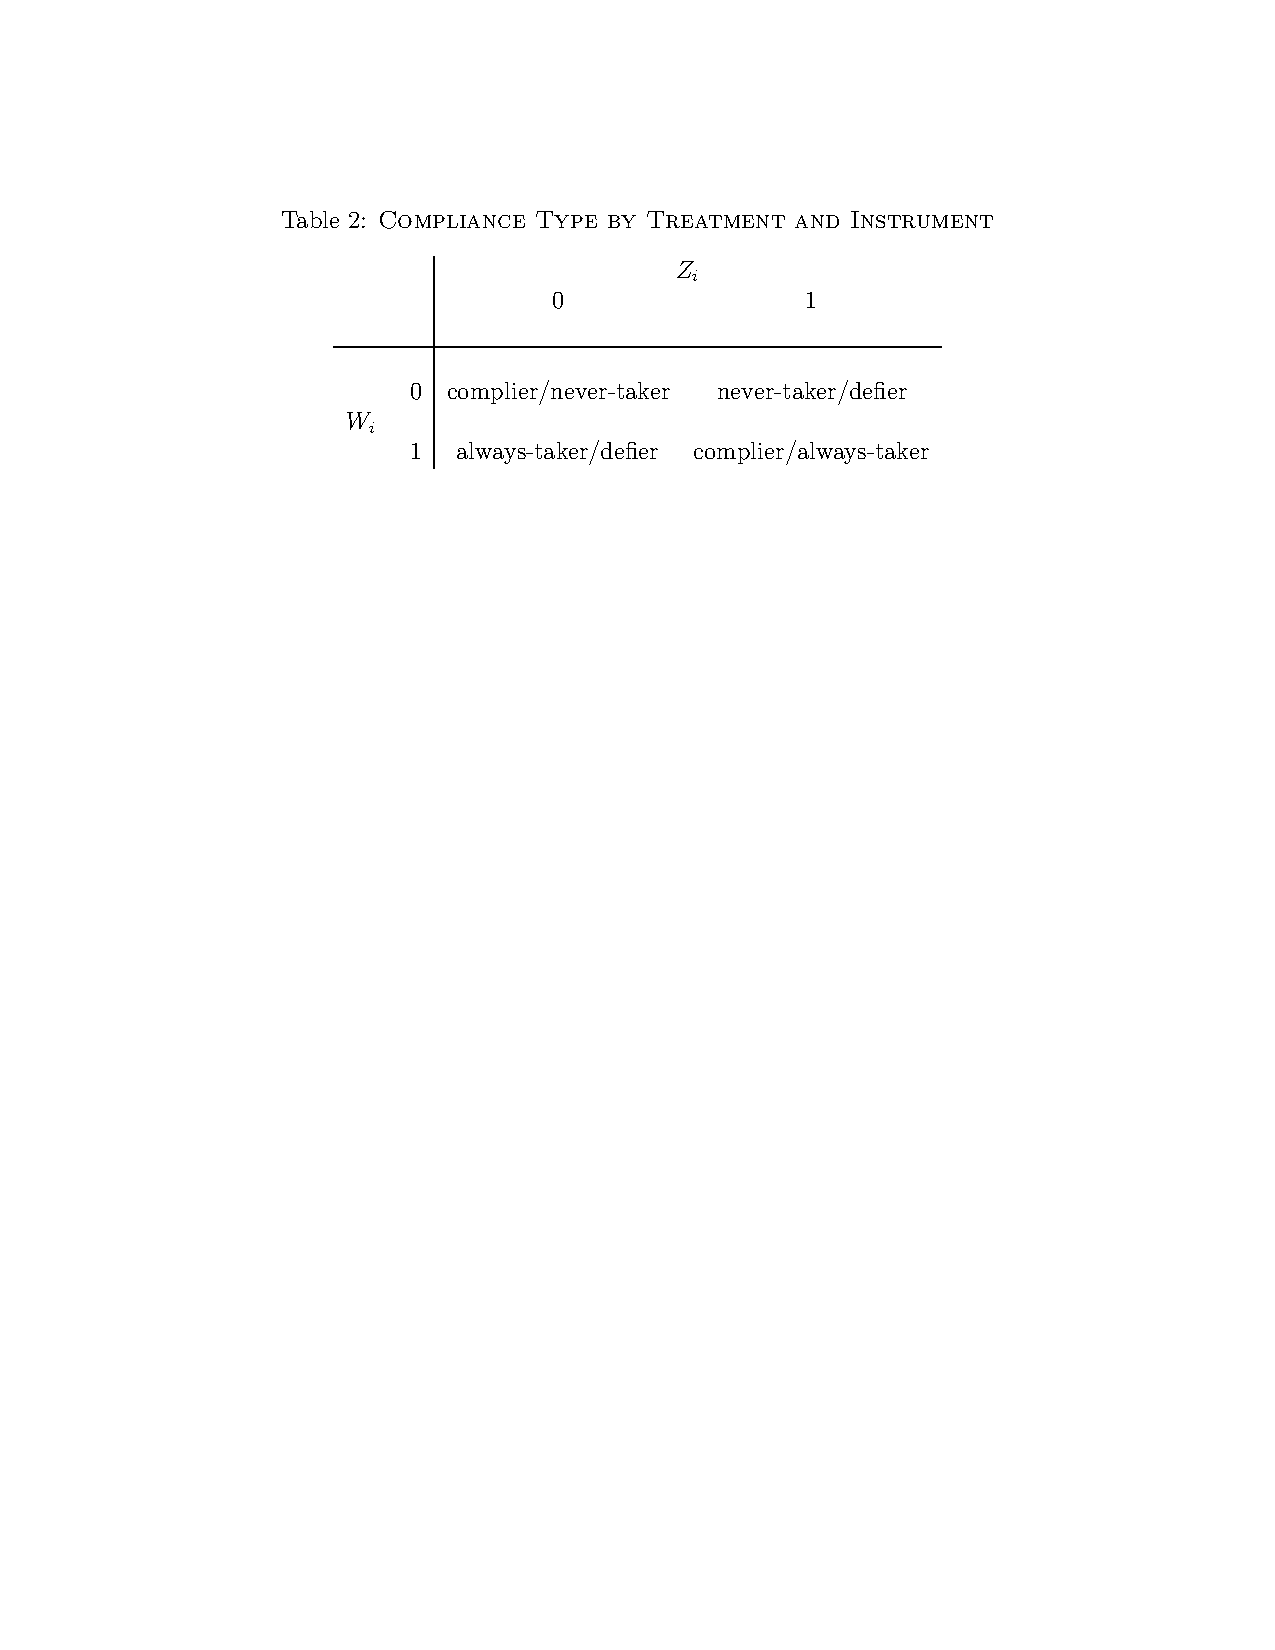
\includegraphics[width=4in]{./resources/imbens2.pdf}
\end{frame}

\begin{frame}
\frametitle{IV Assumptions}
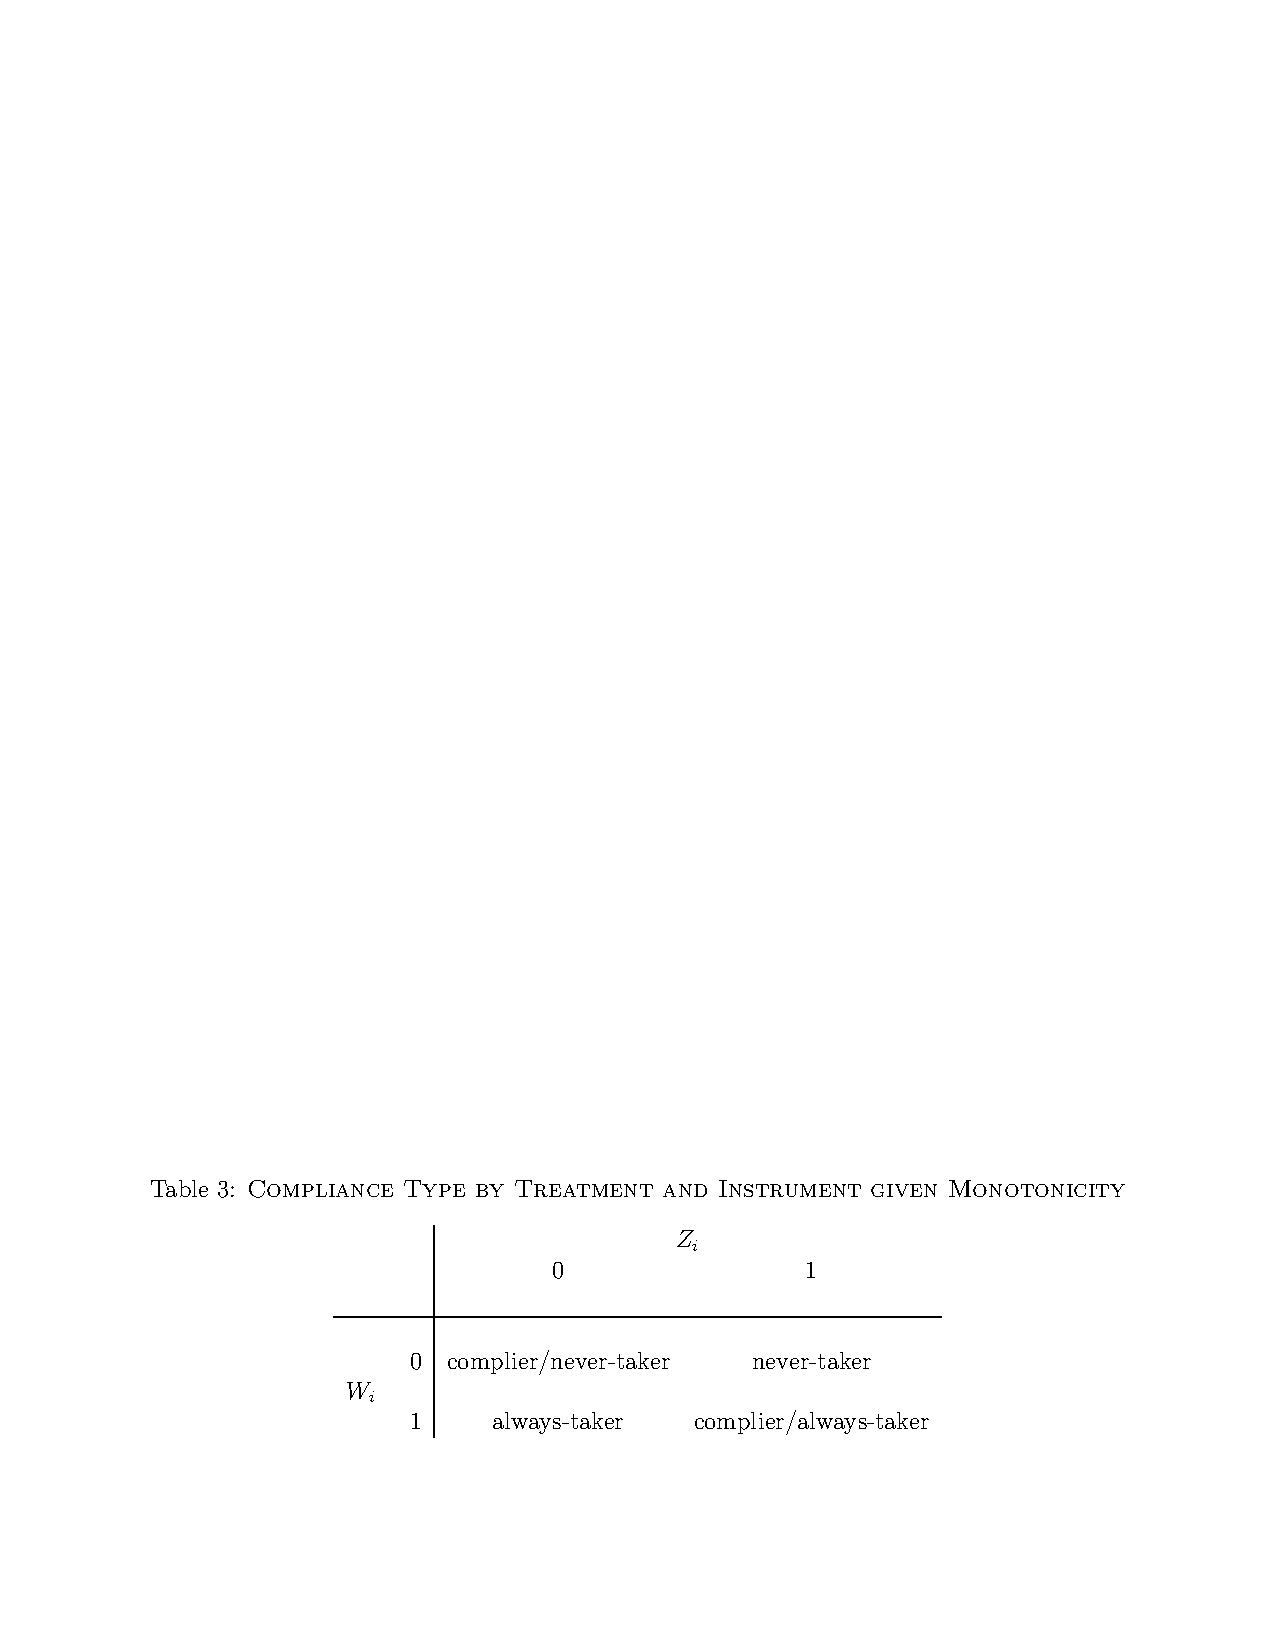
\includegraphics[width=4in]{./resources/imbens3.pdf}
\end{frame}

\begin{frame}
\frametitle{LATE Derivation}
\begin{itemize}
\item We can derive the expression for $\beta_{IV}$ as:
\begin{eqnarray*}
\beta_{IV} = \frac{E[Y_i  | Z_i = 1] - E[Y_i | Z_i = 0] }{E[T_i | Z_i=1 ] - E[T_i | Z_i = 0]} = E[Y_i(1) - Y_i(0) | complier]
\end{eqnarray*}
\item We can derive the expression for $\pi_c$ (the fraction of compliers):
\begin{eqnarray*}
\pi_c = E[T_i | Z_i = 1] - E[T_i | Z_i =0] 
\end{eqnarray*}
\item Proof see Angrist and Imbens
\end{itemize}
\end{frame}

\begin{frame}
\frametitle{How Close to ATE?}
Angrist and Imbens give some idea how close to the ATE the LATE is:
\begin{itemize}
\item $E[Y_i(0) | \text{never-taker}]$ and  $E[Y_i(1) | \text{always-taker}]$ can be estimated from the data
\item Compare these to their respective compliers $E[Y_i(0) | \text{complier}]$, $E[Y_i(1) | \text{complier}]$.
\item When these are close then possibly $ATE \approx LATE$.
\end{itemize}
\end{frame}
\end{comment}


\begin{frame}
\frametitle{How Close to ATE?}
Angrist and Imbens give some idea how close to the ATE the LATE is:
\begin{eqnarray*}
\widehat{\beta}_1^{TSLS} \rightarrow^p \frac{E[\beta_{1i} \pi_{1i}]}{E[\pi_{i1}]} = LATE \\
LATE = ATE + \frac{Cov(\beta_{1i},\pi_{1i})}{E[\pi_{1i}]}
\end{eqnarray*}
\begin{itemize}
\item Weighted average for people with large $\pi_{1i}$.
\item Late is treatment effect for those whose probability of treatment is most influenced by $Z_i$.
\item If you always (never) get treated you don't show up in LATE.
\end{itemize}
\end{frame}

\begin{frame}
\frametitle{How Close to ATE?}
\begin{itemize}
\item With different instruments you get different $\pi_{1i}$ and TSLS estimators!
\item Even with two valid $Z_1, Z_2$
\begin{itemize}
\item Can be influential for different members of the population.
\item Using $Z_1$, TSLS will estimate the treatment effect for people whose probability of treatment $X$ is most influenced by $Z_1$
\item The LATE for $Z_1$ might differ from the LATE for $Z_2$
%\item A J-statistic might reject even if both $Z_1$ and $Z_2$ are exogenous! (Why?).
\end{itemize}
\end{itemize}
\end{frame}


\begin{frame}
\frametitle{Example: Cardiac Catheterization}
\begin{itemize}
\item $Y_i=$ surival time (days) for AMI patients
\item $X_i=$ whether patient received cadiac catheterization (or not) (intensive treatment)
\item $Z_i=$ differential distance to CC hospital
\end{itemize}
\begin{eqnarray*}
SurvivalDays_i &=& \beta_0 + \beta_{1i} CardCath_i + u_i\\
CardCath_i &=& \pi_0 + \pi_{1i} Distance_i + v_i
\end{eqnarray*}
\begin{itemize}
\item For whom does distance have the great effect on probability of treatment?
\item For those patients what is their $\beta_{1i}$?
\end{itemize}
\end{frame}


\begin{frame}
\frametitle{Example: Cardiac Catheterization}
\begin{itemize}
\item IV estimates causal effect for patients whose value of $X_i$ is most heavily influenced by $Z_i$
\begin{itemize}
\item Patients with small positive benefit from CC in the expert judgement of EMT will receive CC if trip to CC hospital is short (\alert{compliers})
\item Patients that need CC to survive will always get it (\alert{always-takers})
\item Patients for which CC would be unnecessarily risky or harmful will not receive it (\alert{never-takers})
\item Patients for who would have gotten CC if they lived further from CC hospital (hopefully don't see) (\alert{defiers})
\end{itemize}
\item We mostly weight towards the people with small positive benefits.
\end{itemize}
\end{frame}


\begin{frame}{Local Average Treatment Effect}
So how is this useful? 
\begin{itemize}
\item It shows why IV can be meaningless when effects are heterogeneous.
\item It shows that if the monotonicity assumption can be justified, IV
estimates the effect for a particular subset of the population.
\item In general the estimates are specific to that instrument and are not
generalisable to other contexts.
\item As an example consider two alternative policies that can increase
participation in higher education.
\begin{itemize}
\item Free tuition is randomly allocated to young people to attend college ($Z_1 = 1$ means that the subsidy is available).
\item The possibility of a competitive scholarship is available for free tuition ($Z_1 = 1$ means that the individual is allowed to compete for the scholarship).
\end{itemize}
\end{itemize} 
\end{frame}


\begin{frame}{Local Average Treatment Effect}
\begin{itemize}
\item Suppose the aim is to use these two policies to estimate the returns to college education. In this case, the pair $\{Y^1, Y^0\}$ are log earnings, the treatment is going to college, and the instrument is one of the two randomly allocated programs.
\item First, we need to assume that no one who intended to go to college will be discouraged from doing so as a result of the policy (monotonicity).
\item This could fail as a result of a General Equilibrium response of the policy; for example, if it is perceived that the returns to college decline as a result of the increased supply, those with better outside opportunities may drop out.
\end{itemize}
\end{frame}

\begin{frame}{Local Average Treatment Effect}
\begin{itemize}
\item Now compare the two instruments.
\item The subsidy is likely to draw poorer liquidity constrained students into college but not necessarily those with the highest returns.
\item The scholarship is likely to draw in the best students, who may also have higher returns.
\item It is not a priori possible to believe that the two policies will identify the same parameter, or that one experiment will allow us to learn about the returns for a broader/different group of individuals.
\end{itemize}
\end{frame}


\begin{comment}
\begin{frame}{Local Average Treatment Effect}
Finally, we need to understand what monotonicity means in terms of restrictions on economic theory. 
\begin{itemize}
\item To quote from Vytlacil (2002) Econometrica:\\
\emph{ ``The LATE assumptions are not weaker than the assumptions of a latent index model, but instead impose the same restrictions on the counterfactual data as the classical selection model if one does not impose parametric functional form or distributional assumptions on the latter.''}
\item This is important because it shows that the LATE assumptions are equivalent to whatever economic modeling assumptions are required to justify the standard Heckman selection model and has no claim to greater generality.
\item On the other hand there are no magical solutions to identifying effects when endogeneity/selection is present; this problem is exacerbated when the effects are heterogeneous and individuals select into treatment on the basis of the returns.
\end{itemize}
\end{frame}
\end{comment}

\subsection{Example: Dobbie et al}

\begin{frame}{Example: Pretrial Detention}
  \begin{itemize}
  \item In US, innocent until proven guilty. 
  \item Some defendants are detained prior to trial. 
  \item Extreme cases are obvious, but lots of discretion in the middle. 
  \item What are the impacts on: 
    \begin{itemize}
      \item time served
      \item future crime
      \item rehabilitation in to workforce
    \end{itemize}  
  \end{itemize}
  \nocite{DobbieGoldinYangBail}
\end{frame}

\begin{frame}
  \frametitle{Example: Pretrial Detention}
  \begin{center}
    
\includegraphics[width=.9\textwidth]{./resources/DobbieAbstract}
  \end{center}  
\end{frame}

\begin{frame}
  \frametitle{Means for detained vs released defendants}
  \begin{center}
    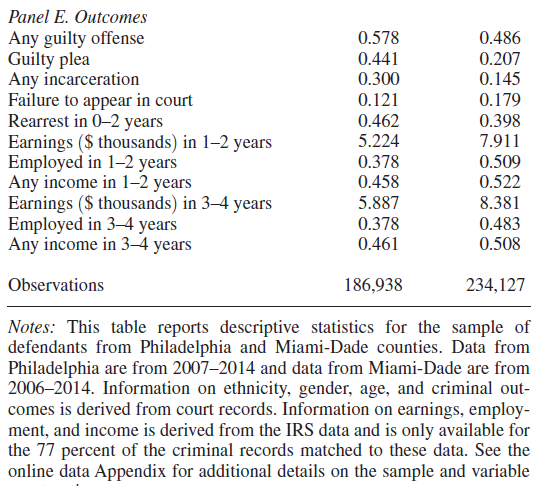
\includegraphics[width=.9\textwidth]{./resources/DobbieStats}
  \end{center}  
\end{frame}

\begin{frame}
  \frametitle{First stage: Judges Matter}
  \begin{center}
    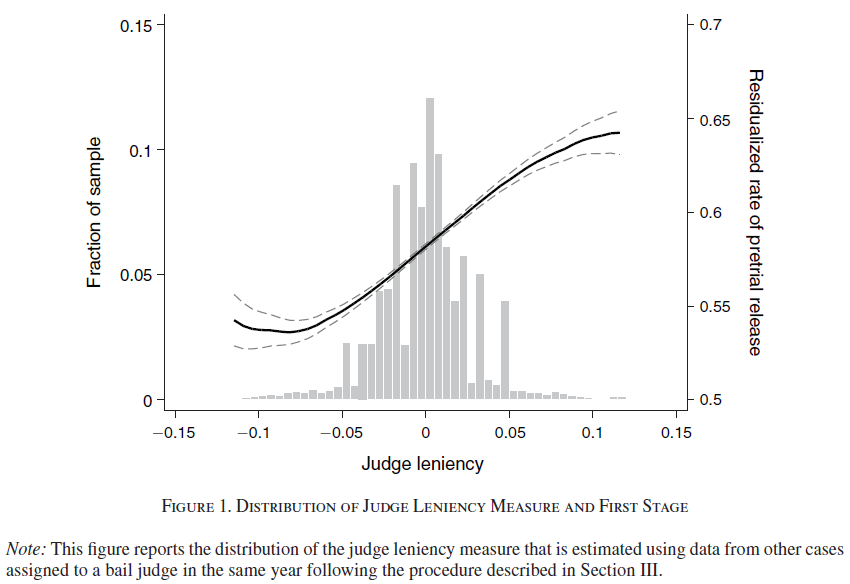
\includegraphics[width=.9\textwidth]{./resources/DobbieFirstStageGraph}
  \end{center}  
\end{frame}

\begin{frame}
  \frametitle{Is assignment random?}
  \begin{center}
    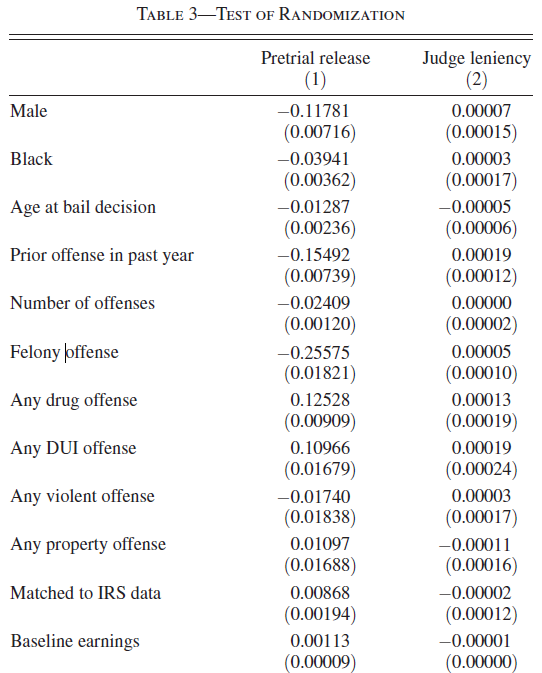
\includegraphics[width=.9\textwidth]{./resources/DobbieRandomization}
  \end{center}  
\end{frame}

\begin{frame}
  \frametitle{Results}
  \begin{center}
    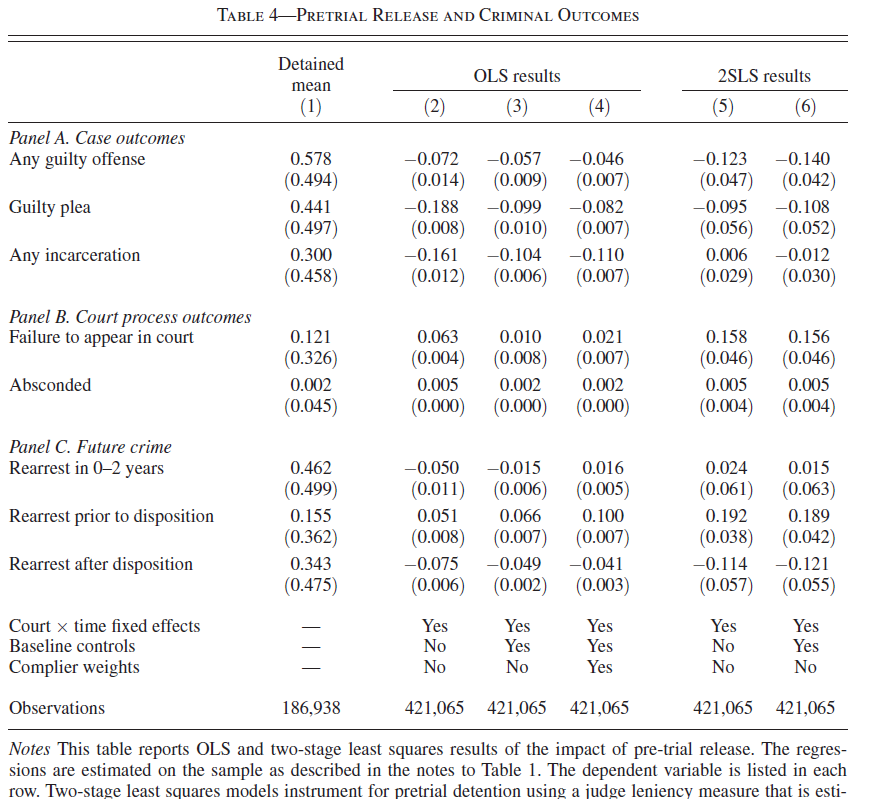
\includegraphics[width=.9\textwidth]{./resources/DobbieResults}
  \end{center}  
\end{frame}

\begin{frame}
  \frametitle{Interpretation: Who is marginal here?}
  \pause 
  \begin{itemize}
    \item Instrument isn't binary here
    \item Thought experiment is the same though: identify which defendants get out under the most lenient judge minus those that get out under the strictest judge 
   \end{itemize}
   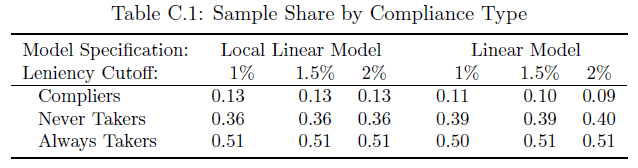
\includegraphics[width=.9\textwidth]{./resources/DobbieCompliers} 
\end{frame}

\begin{frame}
  \frametitle{Who are the compliers?}
  \begin{itemize}
    \item Follow strategy of Dahl et al (QJE 2014)
    \item Estimate complier share by subgroup
   \end{itemize}
   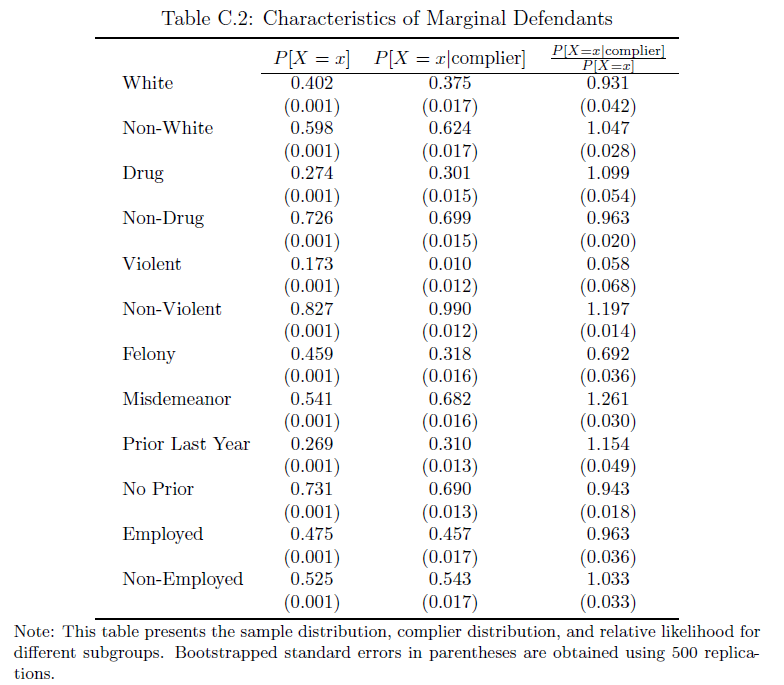
\includegraphics[width=.9\textwidth]{./resources/DobbieComplierStats} 
\end{frame}

\begin{frame}
  \frametitle{How useful is LATE here?}
  \begin{itemize}
    \item What can you do with this estimate?
    \item Is it of policy importance?
   \end{itemize}
\end{frame}

\begin{frame}
  \frametitle{Example: Dams}
  \begin{center}
    
\includegraphics[width=.9\textwidth]{./resources/DamsAbstract}
  \end{center}  
\end{frame}

\begin{frame}
  \frametitle{Example: Dams}
  \begin{itemize}
    \item What is the exclusion restriction here? 
    \item How useful is this LATE?
  \end{itemize}
\end{frame}

\subsection{Weak IVs}

\begin{frame}
  \frametitle{Weak instruments}
  \begin{itemize}
    \item So far we have assumed that the instrument is \alert{relevant}
    $$ cov(Z,W) > 0 $$
    \item Intuitively, if there are no ``compliers'', we can't learn anything from IV. 
    \item In applications, instruments are sometimes barely
    relevant, i.e. $\hat Cov( d z, x) \neq 0$, but it's close.
    \item This leads to: 
    \begin{itemize}
      \item Large finite sample bias of $\hat \beta^{2SLS}$
      \item Inference issues: 
    (wrong standard error, incorrect p-values, incorrect
    confidence intervals)
    \end{itemize} 
   \end{itemize}
\end{frame}

\begin{frame}{}
  \begin{center}
    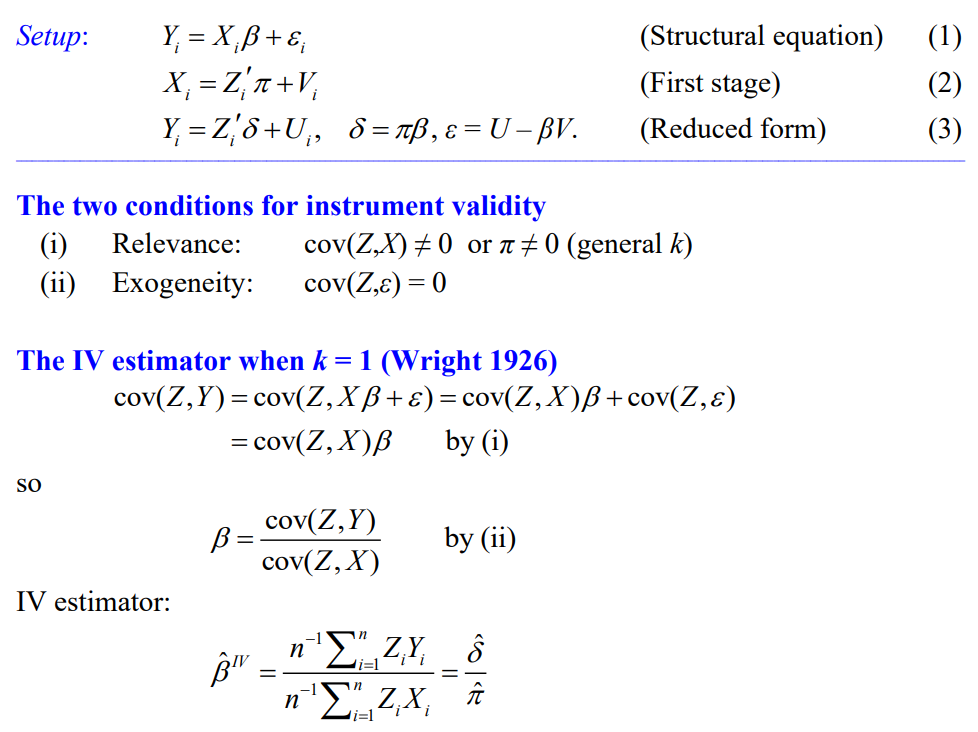
\includegraphics[width=1\textwidth]{./resources/StockNBERIV}
  \end{center}  
\end{frame}


\begin{frame}{}
  \begin{center}
    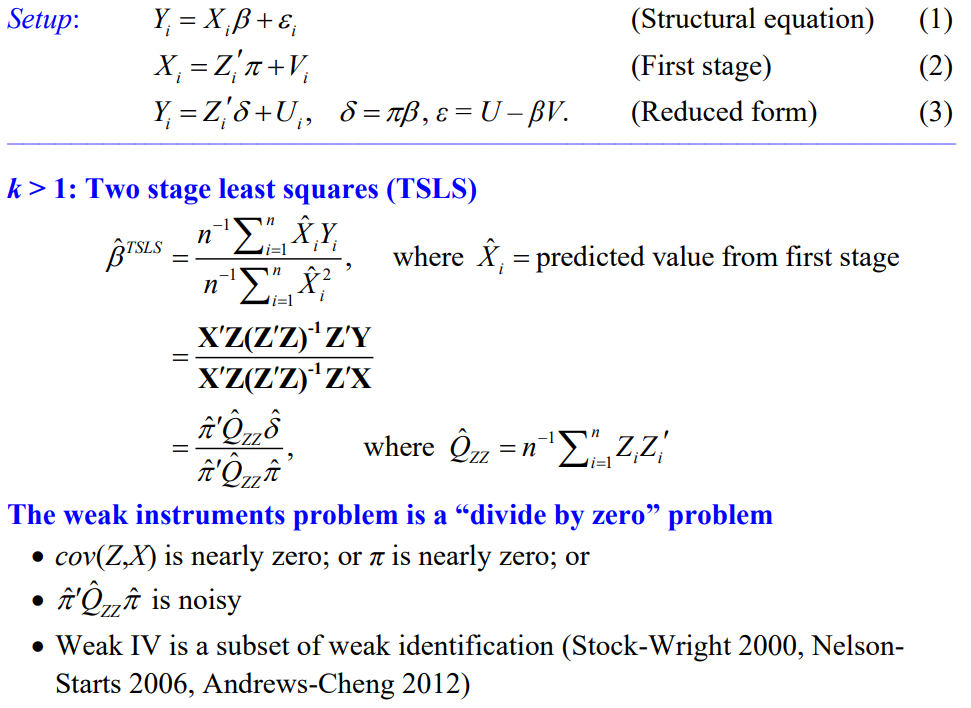
\includegraphics[width=1\textwidth]{./resources/StockNBER2sls}
  \end{center}  
\end{frame}


%http://econ.lse.ac.uk/staff/spischke/ec533/Weak%20IV.pdf
\begin{frame}
  \frametitle{Weak instruments}
  \begin{itemize}
    \item This is an active area of research. See Angrist and Pischke (Ch. 4); or Stock and Andrews 2018 \href{https://www.nber.org/econometrics_minicourse_2018/}{NBER minicourse} for a recent treatment. 
    \item Always report first stage F statistic for significance of
    coefficients on instruments - rule of thumb: F $\ge$ 10 is
    okay (under weak instrument asymptotics, bias
    of 2SLS and is < 10\% when F $\ge$ 10.)
    \item In general, adding weak instruments makes it worse! 
    \item Estimates approach OLS. If instrument doesn't satistfy exclusion restriction, this could be even worse!
   \end{itemize}
\end{frame}

\begin{frame}
  \frametitle{LASSO for selecting instruments}
  \begin{itemize}
    \item Data often gives us many plausibly relevant instruments that satisfy the exclusion restriction. Which should we use?
    \item We know that adding many weak instruments is problematic. 
    \item Intuitively we want something this is highly \textit{predictive} of the endogenous variable. This is what Lasso is good at. \citep{belloni2012sparse}
   \end{itemize}
\end{frame}

\begin{frame}
  \frametitle{Application: Eminent Domain}
  \begin{itemize}
    \item How do changes in the government's ability to appropriate property affect property markets?
    \item Challenge: Changes likely endogenous to the strength of those markets and other economic factors
    \item Even if law changes are endogenous, much of the real world variation comes from court rulings. 
    \item Instrument: Judges
   \end{itemize}
\end{frame}

\begin{frame}
  \frametitle{IV Challenge: Which judges are more inclined to rule for/ against eminent domain?}
  \begin{itemize}
    \item Unlike pretrial detention example, don't have large N of other cases. 
    \item Many judge characteristics: gender, race, religion, political affiliation, whether the judge's bachelor's degree was obtained in-state, whether the bachelor's degree is from a public university, whether the JD was obtained from a public university, and whether the judge was elevated from a district court. 
    \item All are randomly assigned. Which ones are \textit{relevant}? 
   \end{itemize}
\end{frame}

\begin{frame}
  \frametitle{How do we typically proceed here?}
  \begin{itemize}
    \item Pick the ones that make the most sense on intuitive grounds. 
    \item In another paper, Chen and Yeh do exactly this, using  
    \begin{enumerate}
      \item whether a judge did not report a religious affiliation
      \item whether the judge earned her law degree from a public instutition
    \end{enumerate}
    \item Could try other instruments and see if results are "robust" (should they be?)
    \item Could try everything: data mining/ not feasible
    \item Belloni et al. create 140 first stage vars, and let LASSO decide.
    \item Since all satisfy the exclusion restriction (by assumption), this first stage selection has no bearing on second stage intepretation. 
   \end{itemize}
\end{frame}

\begin{frame}
  \frametitle{Results}
  \vspace{-10pt}
  \begin{center}
    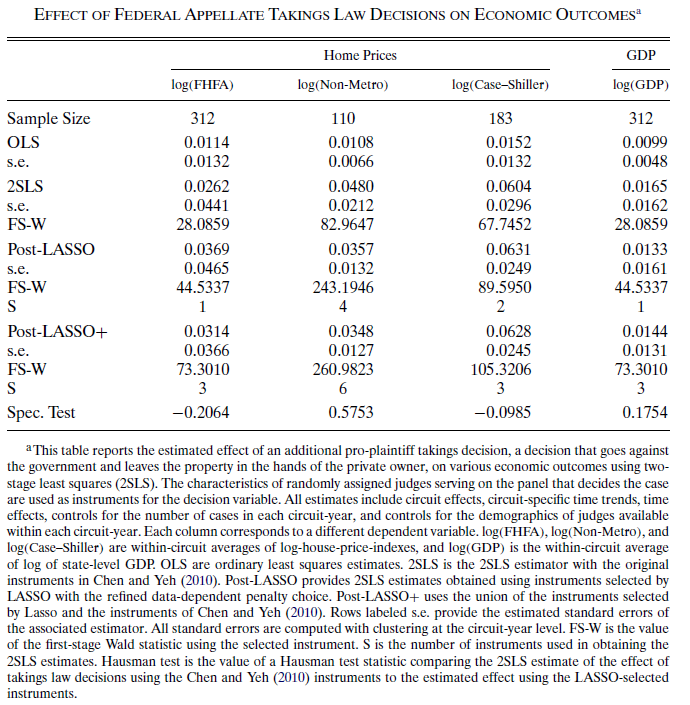
\includegraphics[width=1\textwidth]{./resources/belloniTakingsResults}
  \end{center}  
\end{frame}

\section{RDD}
\begin{frame}{Regression Discontinuity Design}
\begin{itemize}
\item Another popular research design is the \alert{Regression Discontinuity Design}.
\item In some sense this is a special case of IV regression. (RDD estimates a LATE).
\item Most of Chris's slides taken from the JEL Paper by Lee and Lemieux (2010).
\item For an extensive recent treatment, see ``A Practical Introduction to Regression Discontinuity Designs'' (Cattaneo, Idrobo and Titiunik (2019, CUP)) (available \href{https://sites.google.com/site/rdpackages/replication/cit-2019-cup}{here})
\item Matias Catteneo has a number of useful tools (in R and Stata) available on his \href{https://sites.google.com/site/matiasdcattaneo/publications}{website}.
\end{itemize}              
\end{frame}

\begin{frame}{RDD: Basics}
\begin{itemize}
\item We have a \alert{running or forcing variable} $x$ such that 
\begin{eqnarray*}
\lim_{x\rightarrow c^{+}} P(T_i | X_i = x) \neq \lim_{x\rightarrow c^{-}}P(T_i | X_i = x)
\end{eqnarray*}
\item The idea is that there is a \alert{discontinuous jump} in the \alert{probability of being treated}.
\item For now we focus on the \alert{sharp discontinuity}:\\
 $P(T_i | X_i \geq c) =1$ and $P(T_i | X_i < c) =0$
 \item There is no single $x$ for which we observe treatment and control. (Compare to Propensity Score!).
\item The most important assumption is that of \alert{no manipulability} $\tau_i \perp D_i$ in some neighborhood of $c$.
\item Example: a social program is available to people who earned less than \$25,000.
\begin{itemize}              
\item If we could compare people earning \$24,999 to people earning \$25,001 we would have as-if random assignment. (MAYBE)
\item But we might not have that many people...
\end{itemize}
\end{itemize}              
\end{frame}


\begin{frame}{RDD: In Pictures}
\begin{center}
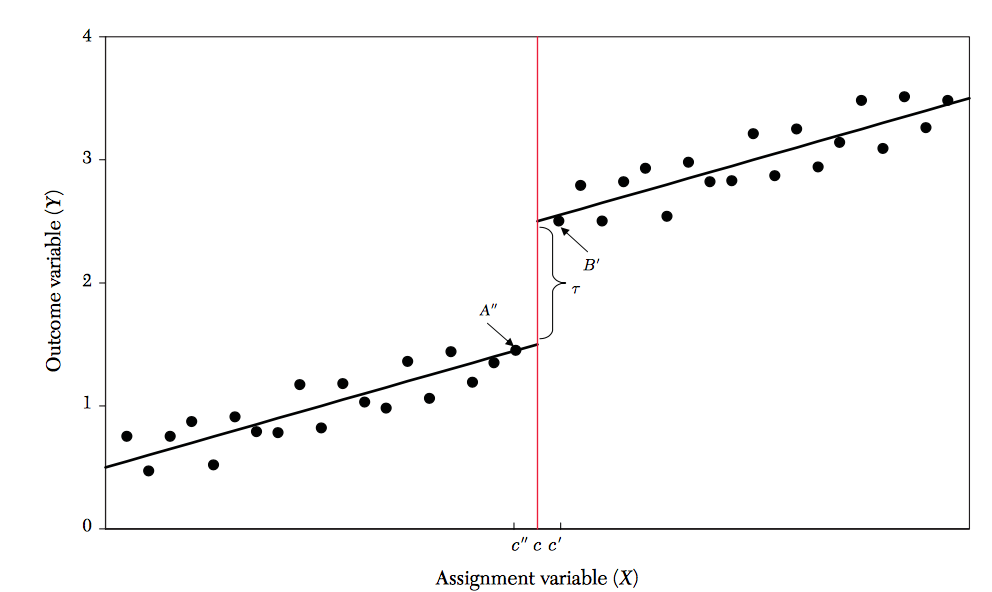
\includegraphics[width= \textwidth]{./resources/ll-fig1}
\end{center}
\end{frame}


\begin{frame}{RDD: Sharp RD Case}
RDD uses a set of assumptions distinct from our LATE/IV assumptions. Instead it depends on \alert{continuity}.
\begin{itemize}
\item We need that $E[Y^{(1)} | X]$ and $E[Y^{(0)} | X]$ both be continuous at $X=c$.
\item People just to the left of $c$ are a valid control for those just to the right of $c$.
\item \alert{This is not a testable assumption} 
  \begin{itemize}
    \item Typically draw pictures of \textit{other} $X$'s at $c$
  \end{itemize}
\item Most basic approach is regression
\begin{eqnarray*}
Y_i = \beta_0 + \tau D_i + X_i \beta + \epsilon_i
\end{eqnarray*} where $D_i = \mathbf{1}[X_i > c]$
\item This puts a lot of restrictions (linearity) on the relationship between $Y$ and $X$.
\end{itemize}
\end{frame}


\begin{frame}{RDD: Nonlinearity}
First thing to relax is assumption of linearity.
\begin{eqnarray*}
Y_i = f(x_i) + \tau D_i  + \epsilon_i
\end{eqnarray*}
\begin{itemize}
\item Two options for $f(x_i)$:
\begin{enumerate}
\item Kernels: Local Linear Regression
\item Polynomials: $Y_i = \beta_0 + \beta_1 x_i + \beta_2 x_i^2 + \cdots + \beta_p x^p + \tau D_i + \epsilon_i$.
\begin{itemize}
\item Actually, people suggest different polynomials on each side of cutoff! (Interact everything with $D_i$).
\end{itemize}
\end{enumerate}
\item Same objective. Want to flexibly capture what happens on both sides of cutoff.
\item Otherwise risk confusing nonlinearity with discontinuity!
\end{itemize}
\end{frame}
	
\begin{frame}{RDD: Kernel Boundary Problem}
\begin{center}
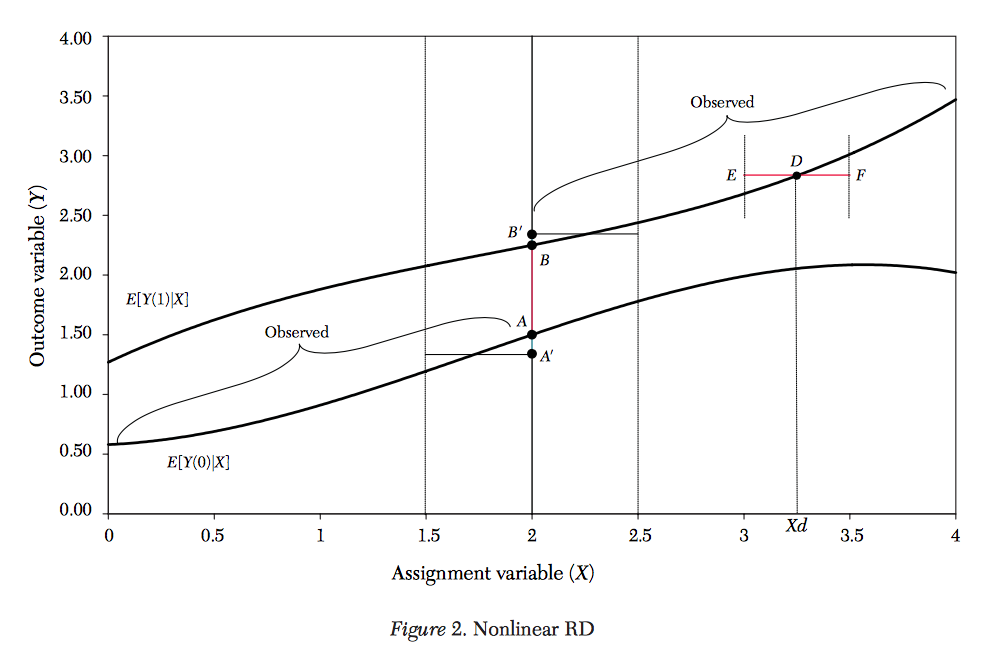
\includegraphics[width=\textwidth]{./resources/ll-fig2}
\end{center}
\end{frame}

\begin{frame}{Important reminder: LOCAL effect}
  \begin{center}
  \includegraphics[width=\textwidth]{./resources/CatteneoLocpoly}
  \end{center}
\end{frame}

\begin{frame}{Bias}
  \begin{center}
  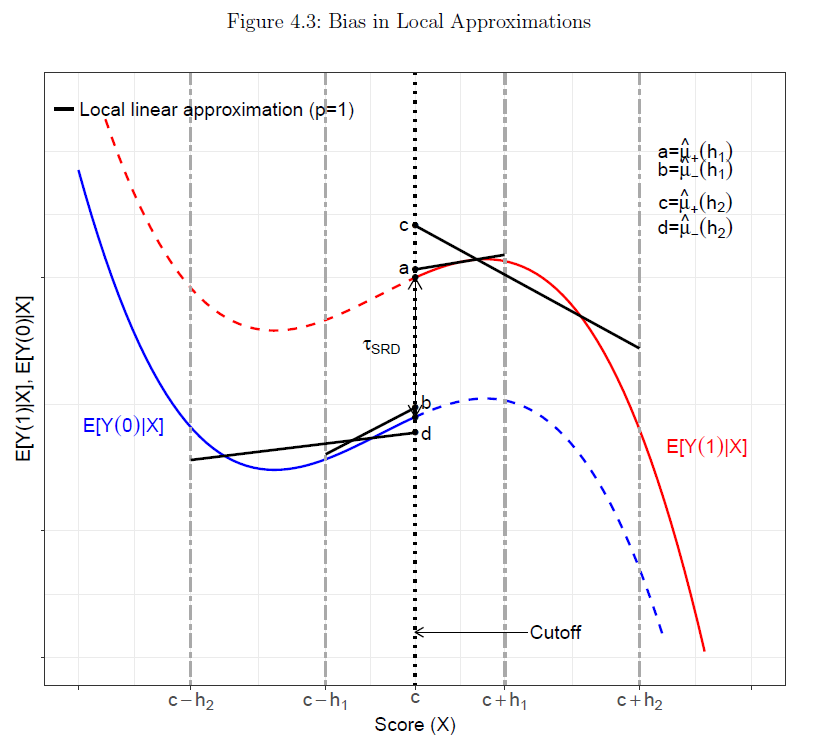
\includegraphics[width=\textwidth]{./resources/CatteneoBias}
  \end{center}
\end{frame}

\begin{comment}
\begin{frame}{Higher order polynomials can be dangerous}
  \begin{center}
  \includegraphics[width=\textwidth]{./resources/CatteneoLocpoly}
  \end{center}
\end{frame}
\end{comment}

\begin{frame}{RDD: Polynomial Implementation Details}
To make life easier:
\begin{itemize}
\item replace $\tilde{x}_i = x_i - c$.
\item Estimate coefficients $\beta$: $(1, \tilde{x}, \tilde{x}^2, \ldots, \tilde{x}^p)$ and\\
 $\tilde{\beta}$: $(D_i, D_i \tilde{x},D_i \tilde{x}^2, \ldots, D_i \tilde{x}^p)$.
 \item Now treatment effect at $c$ just the coefficient on $D_i$. (We can ignore the interaction terms).
 \item If we want treatment effect at $x_i > c$ then we have to account for interactions.
 \begin{itemize}
 \item Identification away from $c$ is somewhat dubious.
\end{itemize}
\item Lee and Lemieux (2010) suggest estimating a coefficient on a dummy for each bin in the polynomial regression $\sum_{k} \phi_k B_k$.
 \begin{itemize}
 \item Add polynomials until you can satisfy the test that the joint hypothesis test that $\phi_1 = \cdots \phi_k= 0$.
\item There are better ways to choose polynomial order...
\end{itemize}
\end{itemize}
\end{frame}

	
\begin{frame}{RDD: Checklist}
Most RDD papers follow the same formula (so should yours)
\begin{itemize}
\item Plot of $P(D | X)$ so that we can see the discontinuity
\item Plot of $E[Y | X]$ so that we see discontinuity there also
\item Plot of $E[W | X ]$ so that we don't see a discontinuity in controls.
\item Density of $X$ (check for manipulation).
\item Show robustness to different ``windows''
\item The OLS RDD estimates
\item The Local Linear RDD estimates
\item The polynomial (from each side) RDD estimates
\item An f-test of ``bins'' showing that the polynomial is flexible enough.
\end{itemize}
Read Lee and Lemieux (2010) before you get started.
\end{frame}

\subsection{Example: Islamic Rule}

\begin{frame}{Application: Meyersson (ECMA, 2014) }
  \begin{itemize}
  \item RQ: Does Islamic political control affect women's empowerment? 
  \item Challenge: Islamic rule endogenous 
  \item Meyerson uses the Lee instrument on 1994 Turkish minicipal elections 
  \item Catteneo et al 2018 use this as a running example to demonstrate how to implement RD (and use their software)
  \end{itemize}
\end{frame}
  
\begin{frame}{Raw vs Local Comparisons}
  \begin{center}
  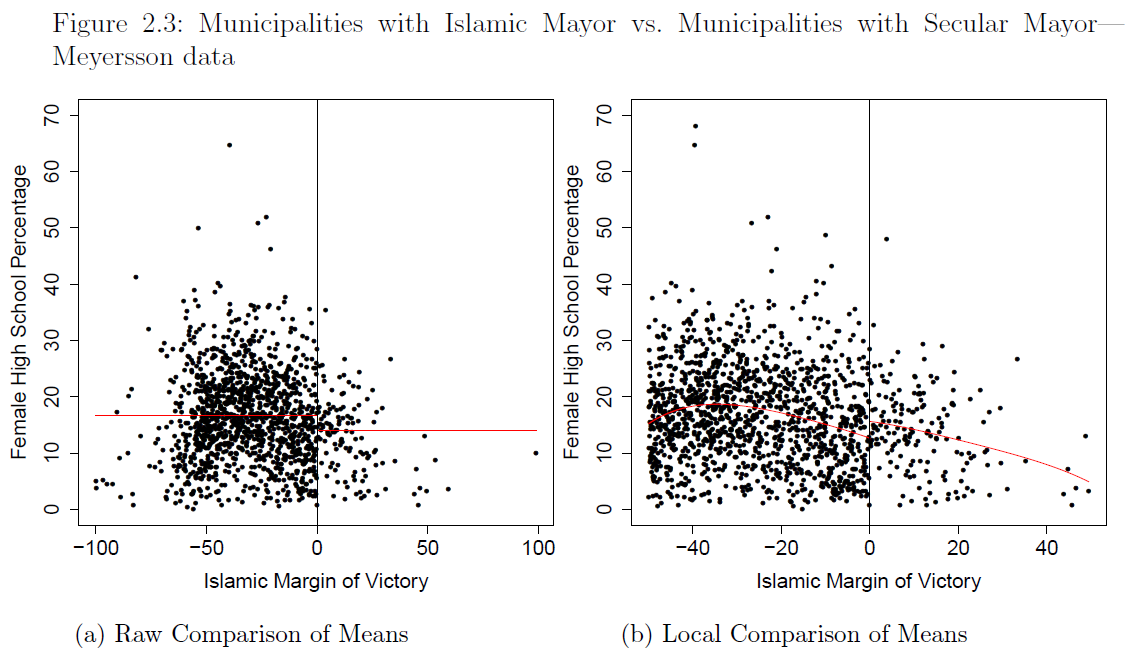
\includegraphics[width=\textwidth]{./resources/CatteneoRawScatter}
  \end{center}
\end{frame}

\begin{frame}{Typically present bincatter}
  \begin{center}
  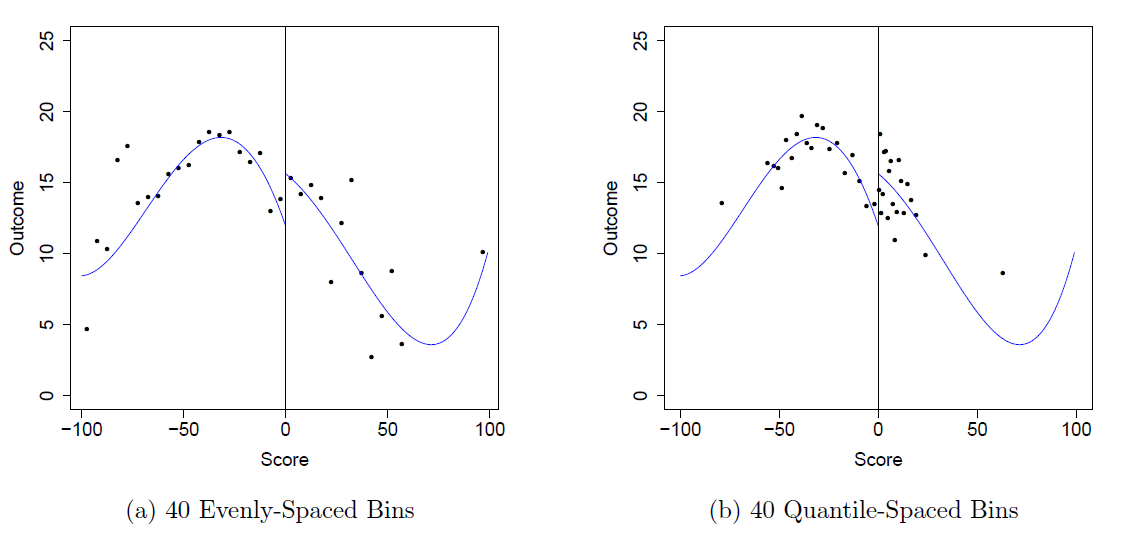
\includegraphics[width=\textwidth]{./resources/CatteneoBinscatter}
  \end{center}
\end{frame}

\begin{frame}{Show other covariates smooth at cutoff}
  \begin{center}
  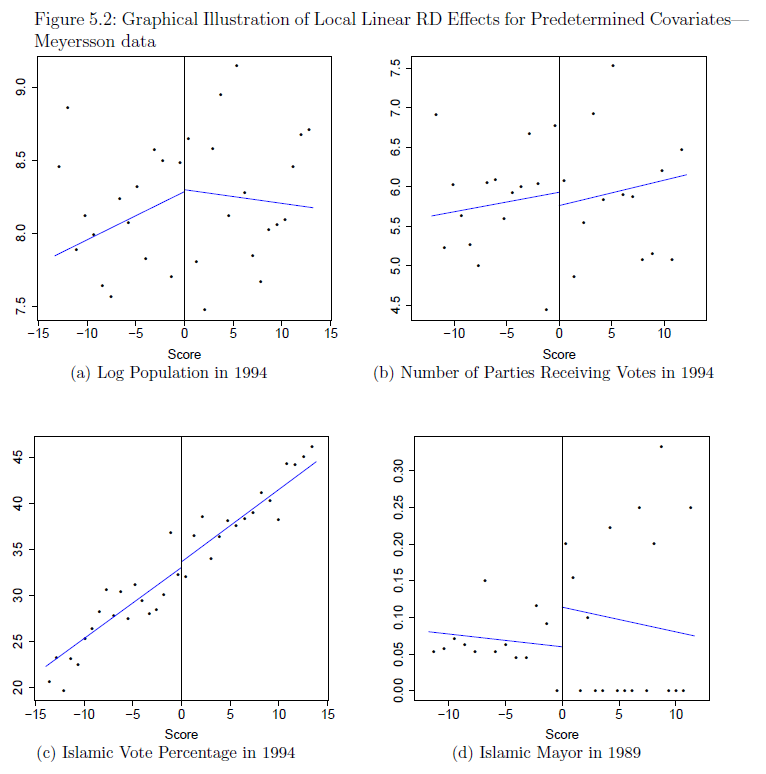
\includegraphics[width=\textwidth]{./resources/CatteneoPredetermined}
  \end{center}
\end{frame}

\begin{frame}{Look for bunching}
  \begin{center}
  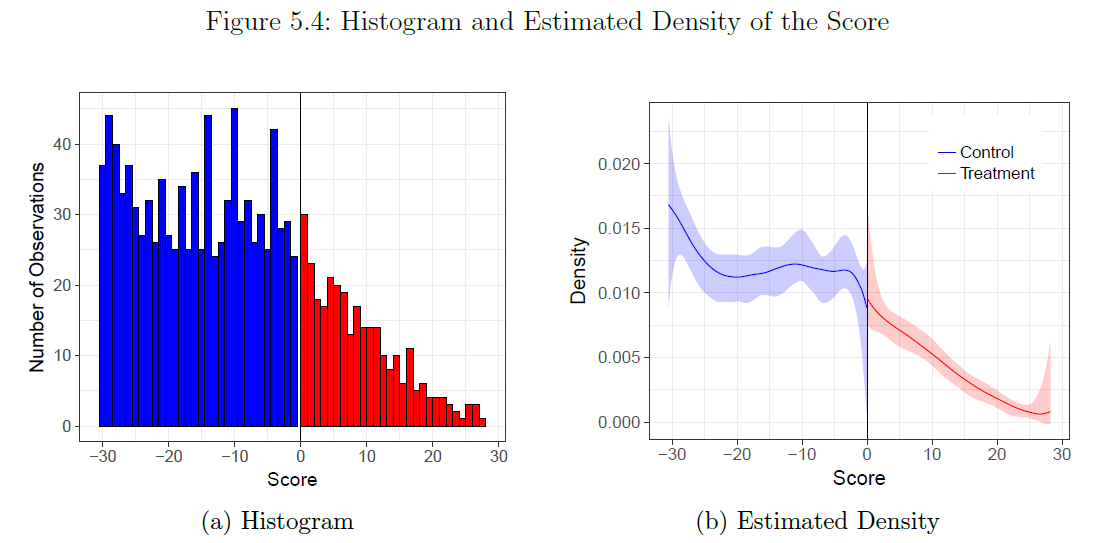
\includegraphics[width=\textwidth]{./resources/CatteneoHistogram}
  \end{center}
\end{frame}

\begin{frame}{How useful is this LATE?}
  \pause
  \begin{center}
  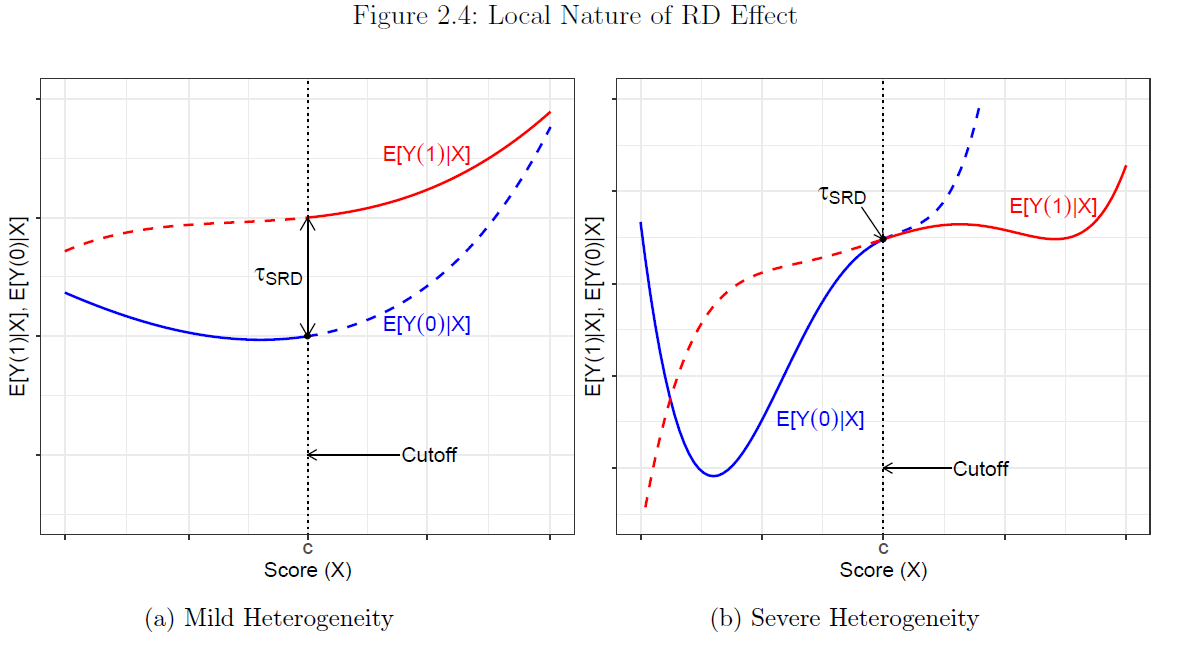
\includegraphics[width=\textwidth]{./resources/CatteneoLocal}
  \end{center}
\end{frame}

\begin{frame}{Other Examples}
Luca on Yelp
\begin{itemize}
\item Have data on restaurant revenues and yelp ratings.
\item Yelp produces a yelp score (weighted average rating) to two decimals ie: $4.32$.
\item Score gets rounded to nearest half star
\item Compare $4.24$ to $4.26$ to see the impact of an extra half star.
\item Now there are multiple discontinuities: Pool them? Estimate multiple effects?
\end{itemize}
\end{frame}

\begin{frame}{Fuzzy RD}
An important extension in the \alert{Fuzzy RD}.   Back to where we started:
\begin{eqnarray*}
\lim_{x\rightarrow c^{+}} P(T_i | X_i = x) \neq \lim_{x\rightarrow c^{-}}P(T_i | X_i = x)
\end{eqnarray*}
\begin{itemize}
\item We need a discontinuous jump in probability of treatment, but it doesn't need to be $0 \rightarrow 1$.
\begin{eqnarray*}
\tau_i(c) = \frac{\lim_{x\rightarrow c^{+}} P(Y_i | X_i = x) - \lim_{x\rightarrow c^{-}}P(Y_i | X_i = x)}{\lim_{x\rightarrow c^{+}} P(T_i | X_i = x) - \lim_{x\rightarrow c^{-}}P(T_i | X_i = x)}
\end{eqnarray*}
\item Under sharp RD everyone was a \alert{complier}, now we have some \alert{always takers} and some \alert{never takers} too.
\item Now we are estimating the treatment effect only for the population of compliers at $x=c$.
\item This should start to look familiar. We are going to do IV!
\end{itemize}
\end{frame}

\begin{frame}{Related Idea: Kinks}
 A related idea is that of \alert{kinks}. 
\begin{itemize}
\item Instead of a discontinuous jump in the outcome there is a discontinuous jump in $\beta_i$ on $x_i$.
\item Often things like tax schedules or government benefits have a kinked pattern.
\end{itemize}
\end{frame}

\section{DiD}
\begin{frame}{Difference in Differences }
\begin{itemize}
\item Sometimes we may feel we can impose more structure on the problem.
\item Suppose in particular that we can write the outcome equation as
\begin{align*}
 Y_{it} =\alpha_i +d_t +\beta_i T_{it} +u_{it}
 \end{align*}
\item In the above we have now introduced a time dimension $t=\{1,2\}$. 
\item Now suppose that $T_{i1}=0$ for all $i$ and $T_{i2}=1$ for a well defined group of individuals in our population.
\item This framework allows us to identify the ATT effect under the assumption that the growth of the outcome in the non-treatment state is independent of treatment allocation:
\begin{align*}
E[Y_{i2}^0 - Y_{i1}^0 | T] = E[Y_{i2}^0 - Y_{i1}^0] 
\end{align*}
\item This is known as \alert{parallel trends}.
\end{itemize}
\end{frame}

\begin{frame}{Before and After} 
An even simpler estimator is the \alert{event study}.
\begin{itemize}
\item We look an outcome before or after an event
\begin{itemize}
\item A news event: the announcement of a merger or stock split.
\item A tax change, a new law, etc.
\end{itemize}
\begin{align*}
E[Y_{i2} - Y_{i1} | T_{i2}=1] & = E[Y_{i2}^1 - Y_{i1}^1 | T_{i2}=1] \\
 &= d_2-d_1 + E[\beta_{i}| T_{i2}=1] 
\end{align*}
\item Except under strong conditions $d_2 = d_1$ we shouldn't believe the results of the before and after estimator.
\item Main Problem: we attribute changes to treatment that might have happened anyway \alert{trend}.
\item e.g: Cigarette consumption drops 4\% after a tax hike. (But it dropped 3\% the previous four years).
\item Also worry about: \alert{anticipation}, \alert{gradual rollout}, etc.
\end{itemize}
\end{frame}

\begin{frame}
  \vspace{-10pt}
  \begin{figure}
  \centering
  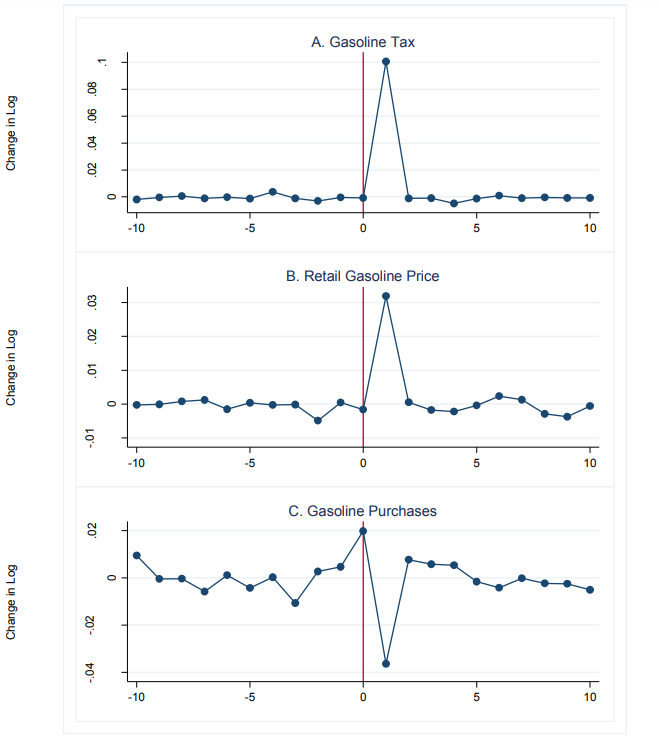
\includegraphics[height=1.05\textheight]{./resources/gasTaxes}
  \end{figure}
\end{frame}


\begin{frame}{Difference in Differences} 
Let's try and estimate $d_2- d_1$ directly and then difference it out. Here we use \alert{parallel trends}:
\begin{align*}
E[Y_{i2}^0 - Y_{i1}^0 | T_{i2}=1]  &= E[Y_{i2}^0 - Y_{i1}^0 | T_{i2}=0] \\
E[Y_{i2} - Y_{i1} | T_{i2}=0] & = d_2-d_1
\end{align*}
We now obtain an estimator for ATT:
\begin{align*}
E[\beta_{i}| T_{i2}=1]  = E[Y_{i2} - Y_{i1} | T_{i2}=1] - E[Y_{i2} - Y_{i1} | T_{i2}=0]  
\end{align*}
which can be estimated by the difference in the growth between the treatment and the control group.
\end{frame}

\begin{frame}{Parallel trends solves a "missing data" problem}
\begin{figure}
\centering
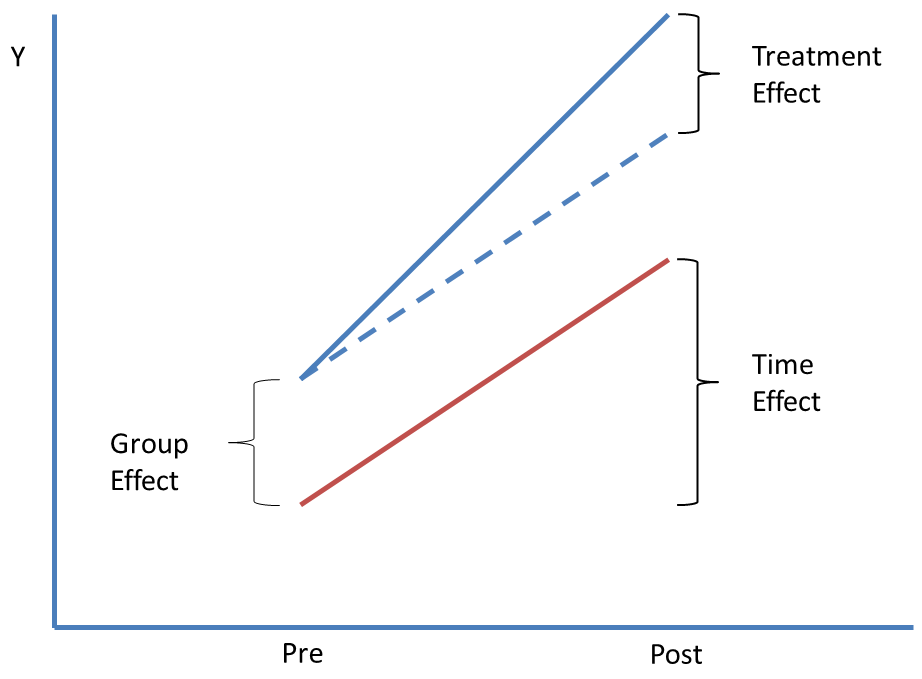
\includegraphics[width=.9\textwidth]{./resources/myDiD}
\end{figure}
\end{frame}

\begin{frame}{Example: Minimum Wage}

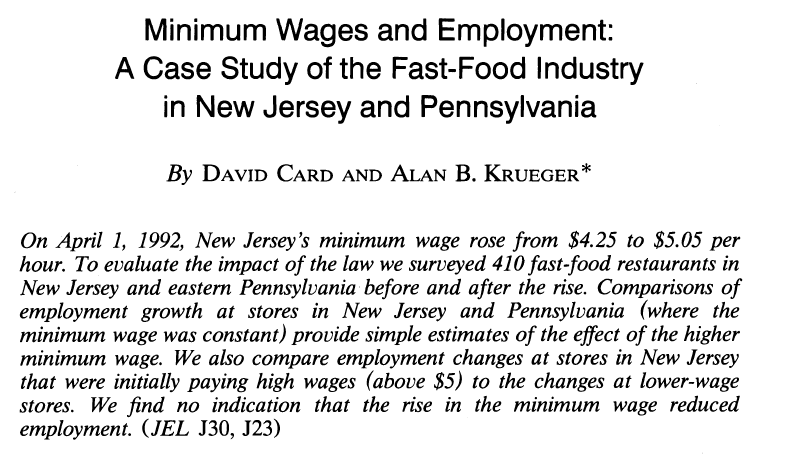
\includegraphics[width=\textwidth]{./resources/CKAbstract}
\end{frame}

\begin{frame}{Example: Minimum Wage}

  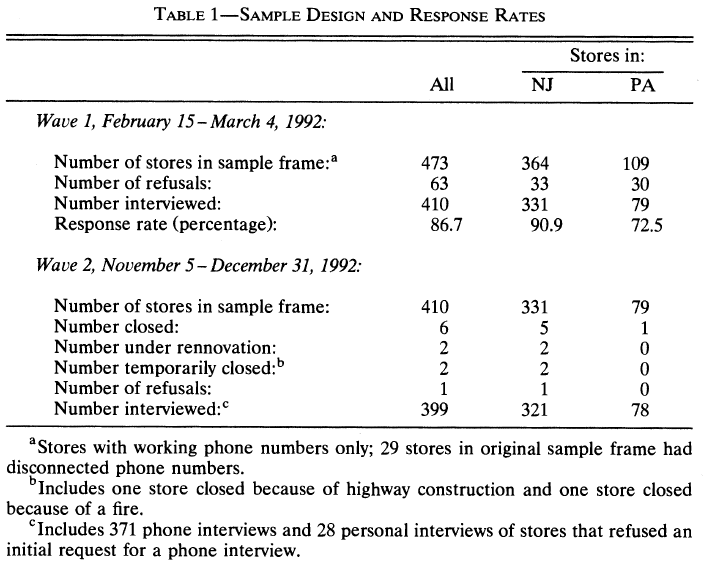
\includegraphics[width=\textwidth]{./resources/CKSumStats}
\end{frame}
  
\begin{frame}
  \vspace{-10pt}
  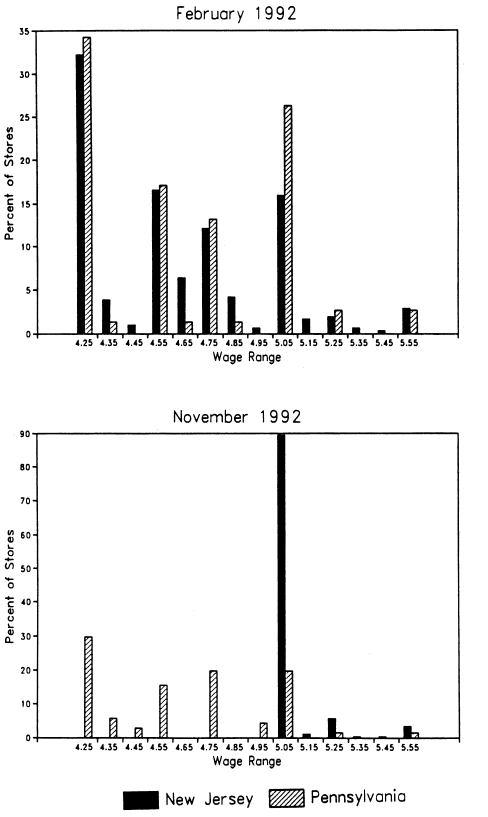
\includegraphics[height=1.1\textheight]{./resources/CKwages}
\end{frame}
  
\begin{frame}
  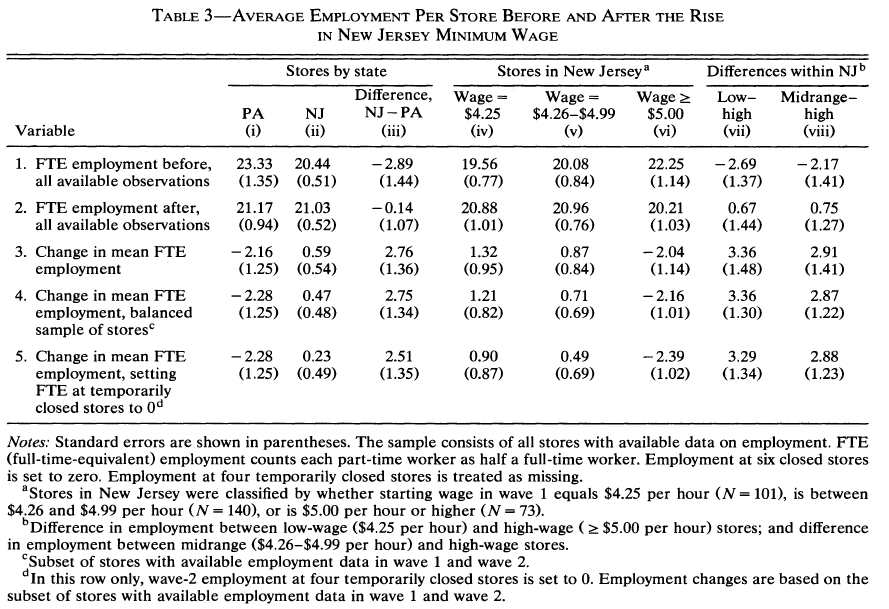
\includegraphics[width=\textwidth]{./resources/CKResults}
\end{frame}


\begin{frame}{Difference in Differences}
  Now consider the following problem:
  \begin{itemize}
  \item Suppose we wish to evaluate a training program for those with low
  earnings. Let the threshold for eligibility be $B$.
  \item We have a panel of individuals and those with low earnings qualify for
  training, forming the treatment group.
  \item Those with higher earnings form the control group. 
  \item Now the low earning group is low for two reasons
  \begin{enumerate}
  \item They have low permanent earnings ($\alpha_i$ is low) - this is accounted for by diff in diffs.
  \item They have a negative transitory shock ($u_{i1}$ is low) - this is not accounted for by diff in diffs.
  \end{enumerate} 
  \item \#2 above violates the assumption {\small $E[Y_{i2}^0 - Y_{i1}^0 | T] = E[Y_{i2}^0 - Y_{i1}^0]$}. 
  \item This is effectively regression to the mean: those unlucky enough to have a bad shock recover and show greater growth relative to those with a good shock. The nature of the bias depends on the stochastic properties of the shocks and how individuals select into training.
  \end{itemize}
  \end{frame} 
  
\begin{comment}
  \begin{frame}{Difference in Differences}
  \begin{itemize}
  \item  \#2 above violates the assumption {\small $E[Y_{i2}^0 - Y_{i1}^0 | T] = E[Y_{i2}^0 - Y_{i1}^0]$}. 
  \item To see why note that those participating into the program are such
  that {\small $Y_{i0}^0 < B$}. Assume for simplicity that the shocks {\small $u$} are {\small $iid$}. Hence {\small $u_{i1} < B- \alpha_i - d_1$}. 
  This implies: 
  {\small $$E[Y_{i2}^0 - Y_{i1}^0 | T=1] = d_2 = d_1 - E[u_{i1}| u_{i1} <  B-\alpha_i - d_1]$$}
  For the control group:
  {\small $$E[Y_{i2}^0 - Y_{i1}^0 | T=1] = d_2 = d_1 - E[u_{i1}| u_{i1} >  B-\alpha_i - d_1]$$}
  \item Hence
  \begin{align*}
  & E[Y_{i2}^0 - Y_{i1}^0 | T=1] - E[Y_{i2}^0 - Y_{i1}^0 | T=0] =\\
  &  E[u_{i1} | u_{i1} >  B-\alpha_i - d_1] - E[u_{i1} | u_{i1} < B-\alpha_i - d_1]  >0
    \end{align*}
   \item This is effectively regression to the mean: those unlucky enough to have a bad shock recover and show greater growth relative to those with a good shock. The nature of the bias depends on the stochastic properties of the shocks and how individuals select into training.
  \end{itemize}
  \end{frame} 
\end{comment}
  
\begin{frame}{Who get's treated?}
\begin{itemize}
\item The assumption on growth of the non-treatment outcome being independent of assignment to treatment may be violated, but it may still be true conditional on $X$.
\item Consider the assumption
$$ E[Y_{i2}^0- Y_{i1}^0 | X,T] = E[Y_{i2}^0- Y_{i1}^0 | X] $$ 
\item This is just matching assumption on a redefined variable, namely the growth in the outcomes. In its simplest form the approach is implemented by running the regression
$$ Y_{it} = \alpha_i + d_t + \beta_i T_{it} + \gamma_t' X_i + u_{it}$$ 
which allows for differential trends in the non-treatment growth depending on $X_i$. More generally one can implement propensity score matching on the growth of outcome variable when panel data is available.
\end{itemize}
\end{frame}

\begin{frame}{DiD with Repeated Cross Sections}
\begin{itemize}
\item Suppose we do not have available panel data but just a random sample from the relevant population in a pre-treatment and a post-treatment period.
\item First consider a simple case where {\small $E[Y_{i2}^0- Y_{i1}^0 | T] = E[Y_{i2}^0- Y_{i1}^0]$}.
\item We need to modify slightly the assumption to
\vspace{-.5pc}
\begin{align*}
E[Y_{i2}^0| \text{\tiny Group receiving training}]&-E[Y_{i1}^0| \text{\tiny Group receiving training in the next period}] \\
&= E[Y_{i2}^0-Y_{i1}^0]  
\end{align*}
which requires additional assumption that the population we will be sampling from does not change composition.
\item We can then obtain immediately an estimator for ATT as
\begin{align*}
&E[\beta_i |T_{i2}=1] \\ 
&= E[Y_{i2}| \text{\tiny Group receiving training}]-E[Y_{i1}| \text{\tiny Group receiving training next period}] \\
&- \{E[Y_{i2} | \text{\tiny Non-trainees}] - E[Y_{i1} | \text{\tiny Group not receiving training next period}]\}
\end{align*}
\end{itemize}
\end{frame}


\begin{frame}{Difference in Differences with Repeated Cross Sections}
\begin{itemize}
\item More generalIy we need an assumption of conditional independence of the form
\begin{align*}
E[Y_{i2}^0 & | X, \text{\tiny Group receiving training}]-E[Y_{i1}^0| X, \text{\tiny Group receiving training next period}] \\
&= E[Y_{i2}^0 | X] - E[Y_{i1}^0 |X]
\end{align*}
\item Under this assumption (and some auxiliary parametric assumptions) we can obtain an estimate of the effect of treatment on the treated by the regression
\begin{align*}
Y_{it} = \alpha_g + d_t + \beta T_{it} + \gamma' X_{it} + u_{it}
\end{align*} 
\end{itemize}
\end{frame}

\begin{frame}{Difference in Differences with Repeated Cross Sections}
\begin{itemize}
\item More generalIy we can first run the regression 
\begin{align*}
Y_{it} = \alpha_g + d_t + \beta (X_{it}) T_{it} + \gamma' X_{it} + u_{it}
\end{align*} 
where $\alpha_g$ is a dummy for the treatment of comparison group, and $\beta (X_{it})$ can be parameterized as $\beta(X_{it}) = \beta' X_{it}$. The ATT can then be estimated as the average of $\beta' X_{it}$ over the (empirical) distribution of $X$.
\item A non parametric alternative is offered by Blundell, Dias, Meghir and van Reenen (2004).
\end{itemize}
\end{frame}

\begin{frame}{DiD vs Fixed Effects}
  \begin{itemize}
  \item What if we have a long panel with many similar changes? 
  \begin{itemize}
    \item Greenstone (2002): Counties move in and out of Clean Air Act
    \item Evans, Ringel, and Stech (1999): Since 1975, more than 200 state cigarette tax changes 
  \end{itemize}
  \item Fixed effects generalize DD with $T > 2$ periods and $J > 2$ groups
  \item Advantage relative to DD: more precise estimates by pooling several
  changes
  \item Disadvantage: fixed effects is a black-box regression, more difficult to
  check trends non-parametrically as with a single change
  \end{itemize}
\end{frame}

\begin{frame}{The best DiD's can be seen graphically}
  \begin{figure}
  \centering
  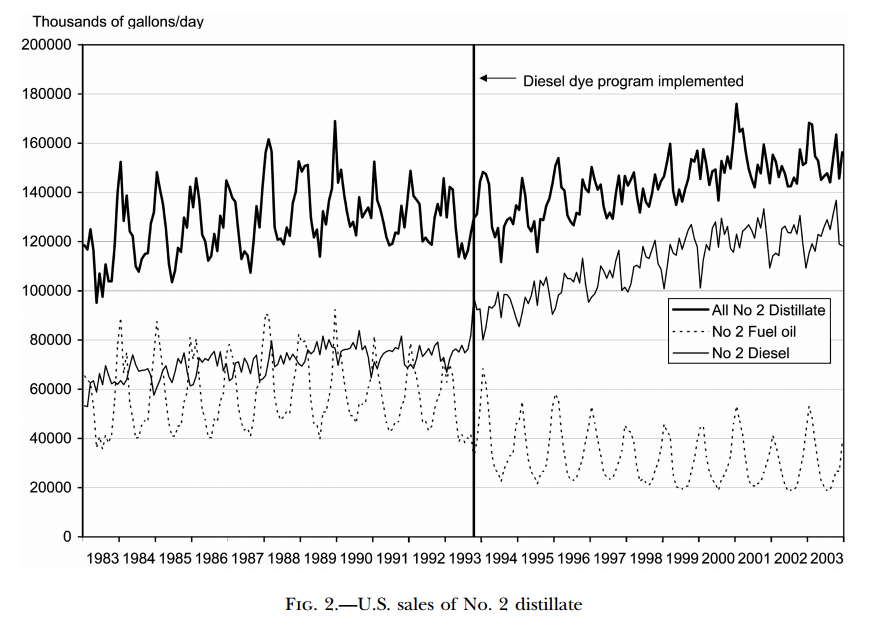
\includegraphics[width=\textwidth]{./resources/muehlegger_dying}
  \end{figure}
\end{frame}

\begin{frame}{What about triple differencing?}
  \begin{itemize}
  \item Sometime we might use a "placebo" DD to make parallel trends more convincing
  \item Example: Imagine a policy which offered STEM outreach to high school girls in Massachusetts 
  \begin{itemize}
    \item Natural DiD control group: boys in MA 
    \item However over time there could be general shifts in the relative outcomes of boys and girls everywhere
    \item Suggest looking at how the difference between boys and girls in MA changed relative to the changes in other states (say RI)
  \end{itemize}
  \item Logically sound, but much harder to see/ validate visually
  \end{itemize}
\end{frame}

\begin{frame}{Difference in Differences and Selection on Unobservables}
\begin{itemize}
\item Suppose we relax the assumption of \emph{no selection} on unobservables. 
\item Instead we can start by assuming that
\begin{align*}
E[Y_{i2}^0 | X,Z] - E[Y_{i1}^0 | X,Z] = E[Y_{i2}^0 | X] - E[Y_{i1}^0 | X]
\end{align*} 
where $Z$ is an instrument which determines training eligibility say but does not determine outcomes in the non-training state. Take $Z$ as binary (1,0).
\item Non-Compliance: not all members of the eligible group ($Z = 1$) will take up training and some of those ineligible ($Z = 0$) may obtain training by other means.
\item A difference in differences approach based on grouping by $Z$ will estimate the impact of being allocated to the eligible group, but not the impact of training itself.
\end{itemize}
\end{frame}

\begin{frame}{Difference in Differences and Selection on Unobservables}
\begin{itemize}
\item Now suppose we still wish to estimate the impact of training on those being trained (rather than just the effect of being eligible)
\item This becomes an IV problem and following up from the discussion of LATE we need stronger assumptions
\begin{itemize}
\item  Independence: for $Z = a, \left\{Y_{i2}^0 - Y_{i1}^0, Y_{i2}^1 - Y_{i1}^1, T(Z=a)\right\}$ is independent of Z.
\item Monotonicity $T_i(1) \ge T_i(0) \, \forall \, i$
\end{itemize}
\item In this case LATE is defined by
 $$\left [E(\Delta Y | Z = 1) - E(\Delta Y | Z = 0)] / [Pr(T(1) = 1) - Pr(T(0) = 1) \right]$$
assuming that the probability of training in the first period is zero.
\end{itemize}              
\end{frame}

\section{Synthetic Controls}

\begin{frame}{Synthetic Controls}
  \begin{itemize}
    \item DiD methods compare two groups before and after some change. 
    \item Challenge: What's a good comparison group? Even if you pick the best available option, might not track eachother that closely even in the pre-period. 
    \item Moreover, if we don't have another untreated group that is well balanced against the treatment group, are we stuck?
    \item Synthetic control methods pick weighted averages from control population to construct better comparisons \citep{abadie2003economic, abadie2010synthetic}
    \item \citet{athey2017state} call this ``arguably the most important innovation in the policy evaluation literature in the past 15 years''.
  \end{itemize}              
\end{frame}

\begin{frame}{Initial motivation: Case studies}
  \begin{itemize}
    \item Often we're interested in the aggregate effects of large, singular policies. 
    \begin{itemize}
      \item What was the impact of MassHealth?
      \item Fukushima 
      \item Terrorism 
      \item German Re-unification
    \end{itemize}  
    \item What would a rigorous "case study" of these look like?
  \end{itemize}              
\end{frame}

\begin{frame}{ADH (JASA 2010)}
  \begin{itemize}
  \item Consider a panel with $J+1$ units observed for $t=1,2,...,T$ periods.
  \item Unit 1 exposed to treatment in period $T_0$ (continues to $T$)
  \item Synthetic control estimator is 
  $$ \hat \alpha_{1t} = Y_{1t} - \sum^{J+1}_{j=2}w_j^{*}Y_{jt} $$ where $w$ is a collection of weights. 
  \item In \cite{abadie2010synthetic} the (non-negative) weights are chosen to minimize the distance between some chosen vector of preintervention characteristics (and sum to one). 
  \item Subsequent literature has relaxed these. 
  \end{itemize}
\end{frame}

\begin{frame}{ADH Example: CA Prop 99}
  \begin{itemize}
  \item Anti cigarette law in CA in 1988
  \begin{itemize}
    \item increased state excise tax by 25 cents per pack
    \item earmarked the tax revenues to health and anti-smoking education budgets
    \item funded anti-smoking media campaigns
    \item spurred local clean indoor-air ordinances throughout the state
  \end{itemize}
  \item What was the net effect on sales?
  \end{itemize}
\end{frame}

\begin{frame}
  \frametitle{Sales were trending down everywhere}
  \begin{center}
    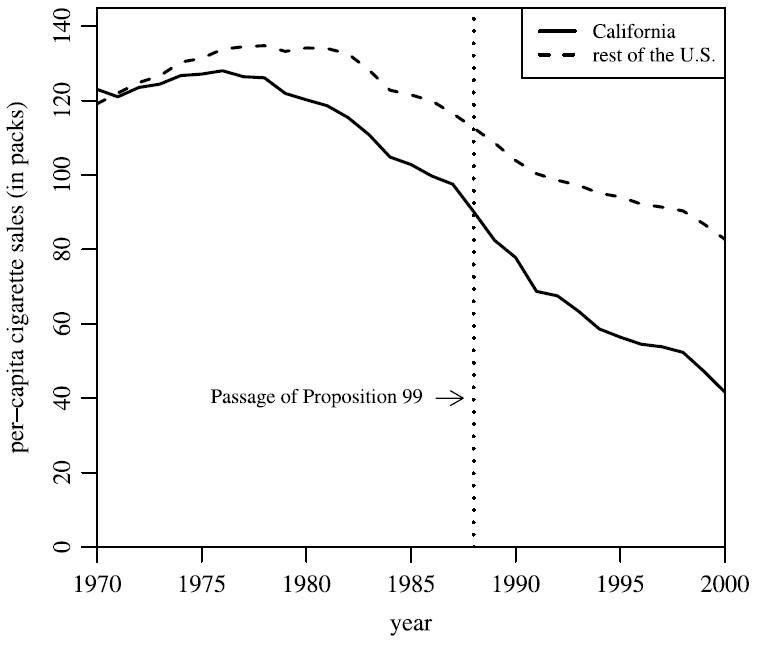
\includegraphics[width=.85\textwidth]{./resources/ADHCAvsUS}
  \end{center}  
\end{frame}

\begin{frame}
  \frametitle{What does synthetic CA look like?}
  \vspace{-15pt}
  \begin{center}
    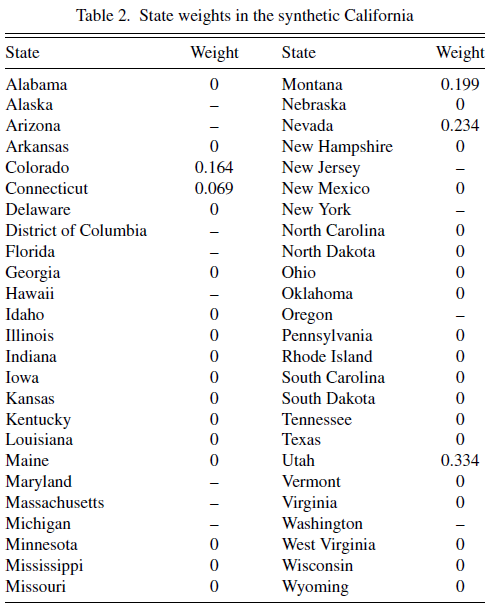
\includegraphics[height=.95\textheight]{./resources/ADHWeights}
  \end{center}  
\end{frame}

\begin{frame}
  \frametitle{Balance Acheived}
  \begin{center}
    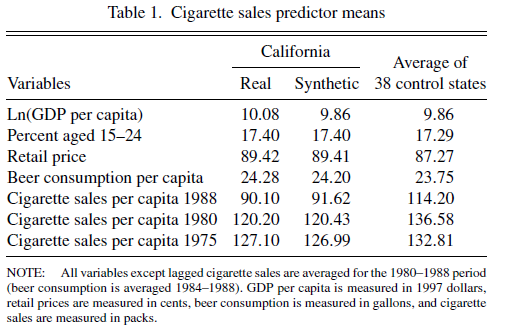
\includegraphics[width=.9\textwidth]{./resources/ADHSumStats}
  \end{center}  
\end{frame}

\begin{frame}
  \frametitle{}
  \begin{center}
    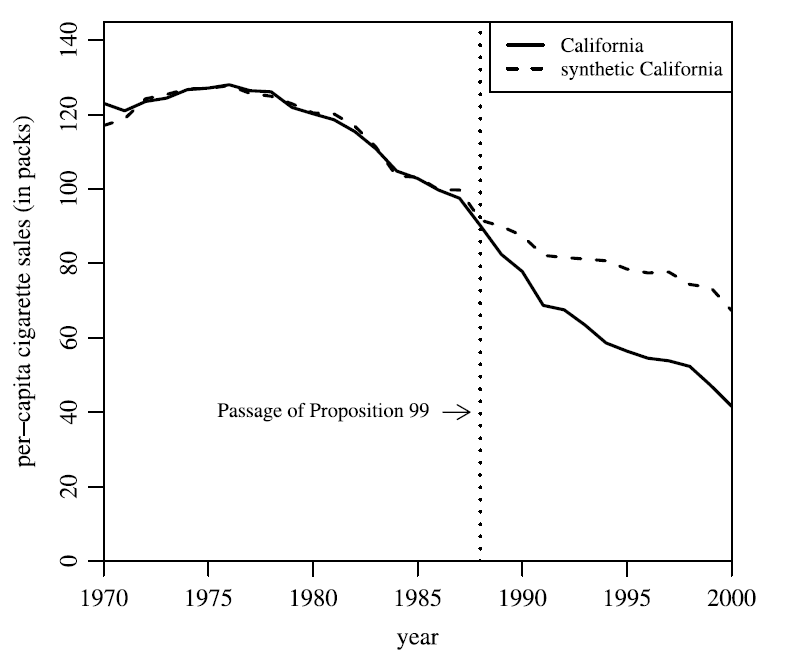
\includegraphics[width=.9\textwidth]{./resources/ADHCAsynth}
  \end{center}  
\end{frame}

\begin{frame}
  \frametitle{Parallel trends acheived by contstruction}
  \vspace{-10pt}
  \begin{center}
    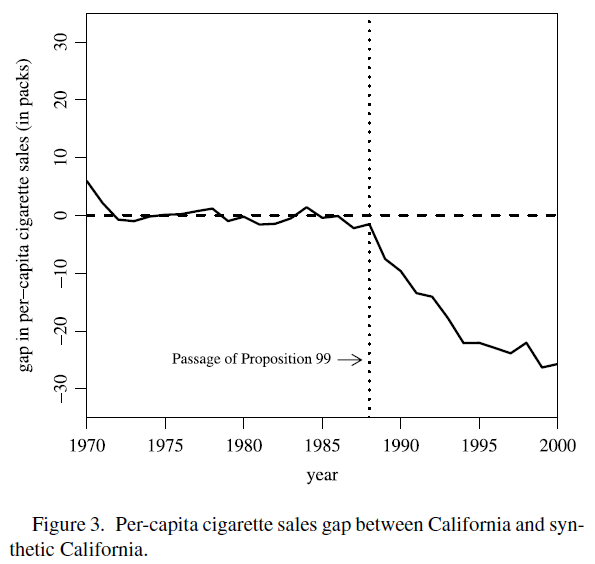
\includegraphics[width=.9\textwidth]{./resources/ADHSdifftrends}
  \end{center}  
\end{frame}

\begin{frame}
  \frametitle{What about inference}
  \begin{itemize}
    \item SE's typically reported reflect uncertainty in sample relative to aggregate population. 
    \item ADH propose using a placebo test to assess null of no change in CA.
    \item Steps:
      \begin{enumerate}
        \item Randomly select one of the other $J$ control units / time cutoffs and declare it treated. 
        \item Construct synthetic controls and estimate ATT. 
        \item Repeat many times
      \end{enumerate}
    \item Since none of these units are actually treated, this test distribution simulates distribution of the differences relative to the synthetic control under the true null of no effect. 
  \end{itemize}
\end{frame}

\begin{frame}
  \frametitle{}
  \begin{center}
    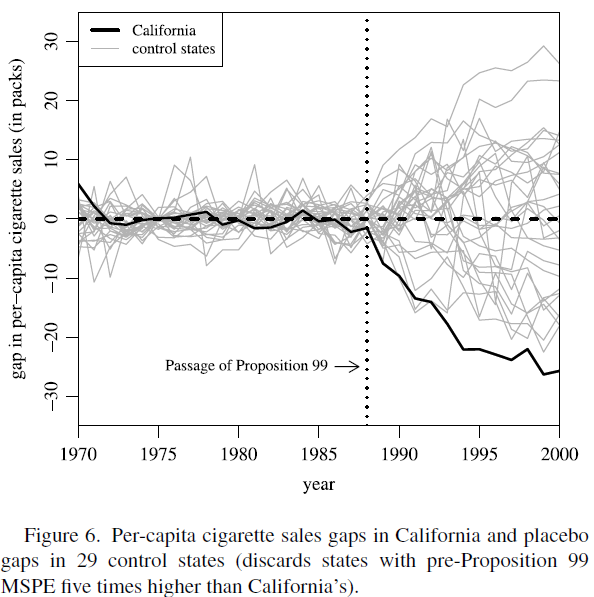
\includegraphics[width=.85\textwidth]{./resources/ADHPlacebo}
  \end{center}  
\end{frame}

\begin{frame}
  \frametitle{}
  \begin{center}
    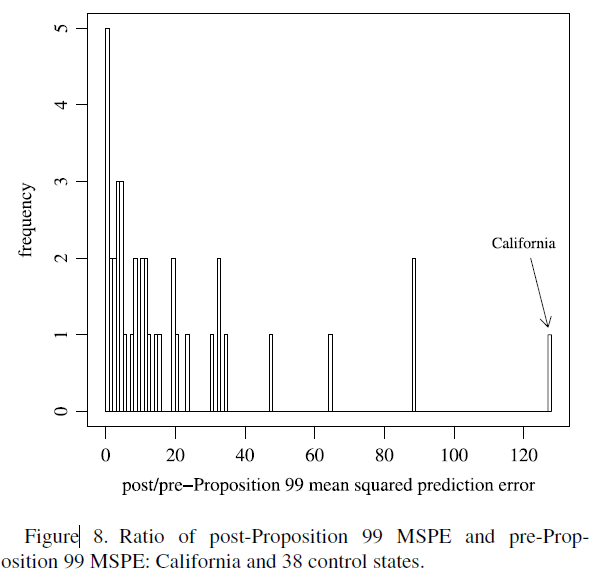
\includegraphics[width=.9\textwidth]{./resources/ADHPredictionErrors}
  \end{center}  
\end{frame}


\begin{frame}
  \frametitle{A synthesis of approaches}
  \begin{itemize}
    \item \citet{DoudchenkoImbensSynth} attempt to synthesize several of the approaches discussed so far balancing (matching), regression, DiD, synthetic controls. 
    \item These methods can be recast as trying to impute the untreated outcome for treated unit $0$ to estimate $\hat \tau_{0,T} = Y_{0,T}(1) - \hat Y_{0,T}(0)$
    \item many impose the linear structure $$ \hat Y_{0,T}(0) = \mu + \sum_{i}^{N}w_i \dot Y_{i,T}^{obs} $$
  \end{itemize}
\end{frame}
    
\begin{frame}
    \frametitle{DI consider a series of contstraints}
  \begin{enumerate}
    \item no intercept: $\mu = 0$
    \item adding up: $ \sum_i^N w_i = 1$
    \item non-negativity: $w_i > 0$ 
    \item exact balancing: $Y_{t,pre}^{obs} = \mu + w^T\mathbf{Y_{c,pre}^{obs}}$
    \item constant weights: $w_i = \bar w$ 
  \end{enumerate}

  \begin{itemize}
    \item Assumptions 1-3 are imposed by ADH 
    \item No intercept actually precludes defining feature of DiD
    \item Contstant weights implicit when number of control units is large
    \item Other useful features of an objective function:
    \begin{itemize}
      \item match pre period \textit{outcomes} well 
      \item small number of features 
      \item non-disperse set of parameters
    \end{itemize}
    \item All of these generally suggest regularization. 
  \end{itemize}
\end{frame}

\begin{frame}
  \frametitle{}
  \begin{center}
    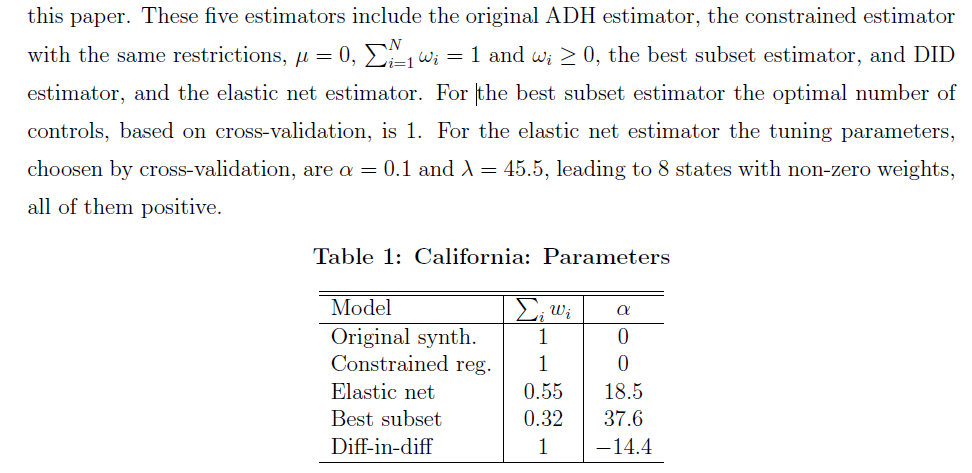
\includegraphics[width=\textwidth]{./resources/DI_CAweights}
  \end{center}  
\end{frame}

\begin{frame}
  \frametitle{}
  \begin{center}
    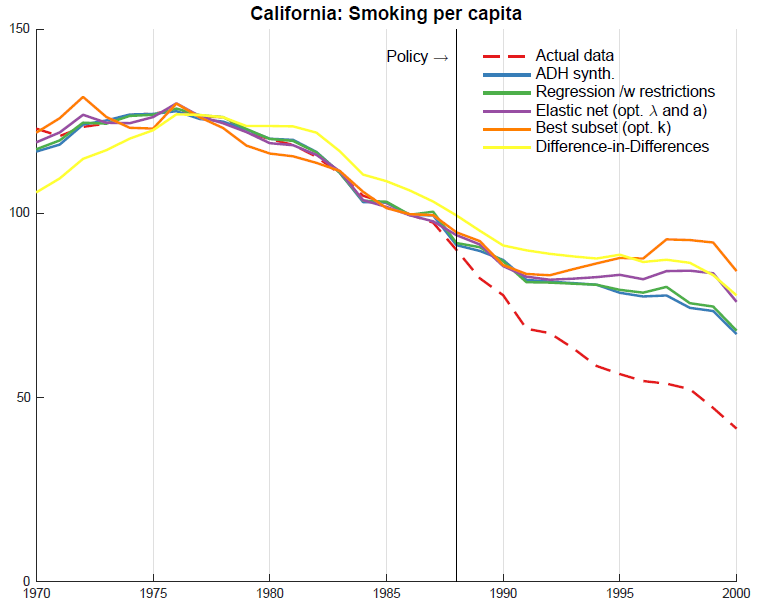
\includegraphics[width=\textwidth]{./resources/DI_CA_trends}
  \end{center}  
\end{frame}

\begin{frame}
  \frametitle{}
  \begin{center}
    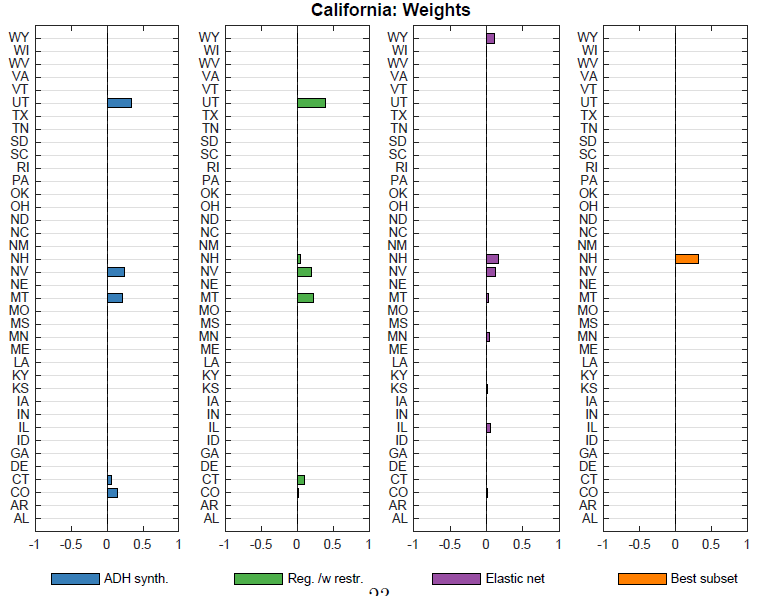
\includegraphics[width=\textwidth]{./resources/DI_CAstates}
  \end{center}  
\end{frame}



\section{MTE}

\begin{frame}
  \frametitle{Treatment effect heterogeneity}
  \begin{itemize}
    \item Consider a binary treatment $T_i$
    \item Potential outcomes
      \begin{eqnarray*}
      Y_{0i} &=& \mu_{0}(X_i) + U_{0i} \\
      Y_{1i} &=& \mu_{1}(X_i) + U_{1i}\\
      \end{eqnarray*}
    \item $\mu_j(x)$ represents the average outcome for individuals with observables $x$, and conditional mean zero $U_{ji}$ captures unobserved heterogeneity (assumed to be additively separable)
    \item Individual treatment effect $\tau_i = Y_{1i} - Y_{0i}$ 
    \item ATE averages $\tau_i$ over entire population.
    \item ATT / ATU averges over those who recieved / didn't recieve the treatment (somehow)
    \item LATE averages for those induced to switch due to an instrument 
  \end{itemize}
\end{frame}

\begin{frame}{One quantity to rule them all: MTE}

 Their approach is known as the \alert{marginal treatment effect} or MTE
\begin{itemize}
\item \citet{heckman2005structural} provide a unifying non-parametric framework to categorize all of these effects
\item Key insight is that those are all averages over different margins. 
\item Define the \alert{marginal treatment effect} as the average treatment effect at the margin. The MTE isn't a number it is a \alert{function}.
\item All of the other objects (LATE, ATE, ATT, etc.) can be written as integrals (weighted averages) of the MTE.
\item The idea is to bridge the treatment effect parameters (stuff we get from running regressions) and the structural parameters: features of $f(\tau_i)$.
\end{itemize}
\end{frame}

\begin{frame}
  \frametitle{Setup: Selection into treatment}
  \vspace{-8pt}
  Consider the latent variable discrete choice problem 
  \begin{itemize}
    \item Decision utility $$T_i^* = \mu_T(X_i,Z_i) - V_i$$ depends on at least one instrument $Z$ which does not affect potential outcomes. 
    \item $V_i$ represents the unobserved disutility of decision. 
    \item $T_i = 1$ if $T_i^* \ge 0$ 
  \end{itemize}
  
  Example: Let $\tau_i$ be lifetime earnings with and without college. 
    \begin{itemize}
      \item Costs of attending $C_i = w_0 + \gamma'z_i + v_{i}$
      \item Rational students attend if $$ \tau_i - [w_0 + \gamma'z_i + v_{i}] > 0$$
      \item If we could condition on marginal students, 
          $$v_{i} = \tau_i - [w_0 + \gamma'z_i]$$
      we'd be able to pin down the treatment effect at a given $Z_i$   
    \end{itemize}
\end{frame}


\begin{frame}
  \frametitle{HV Roy Model}
  \begin{center}
    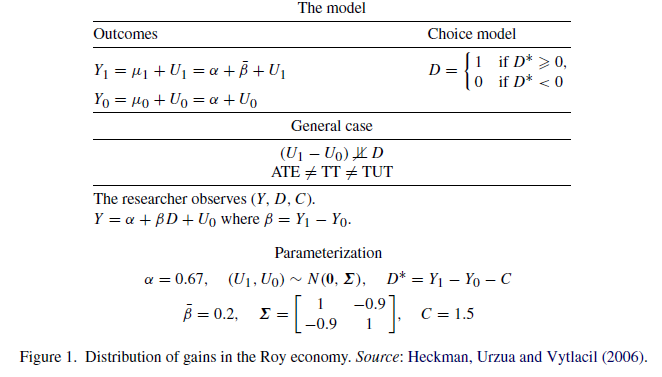
\includegraphics[width=.9\textwidth]{./resources/HVRoyModel}
  \end{center}  
\end{frame}


\begin{frame}
  \frametitle{HV Roy Model}
  \begin{center}
    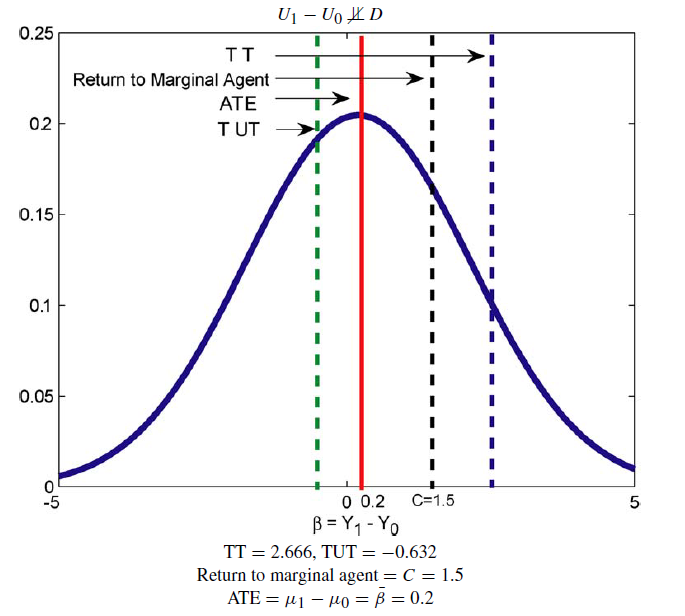
\includegraphics[width=.85\textwidth]{./resources/HVRoyDist}
  \end{center}  
\end{frame}

\begin{frame}
  \frametitle{Propensity score}
  \begin{itemize}
    \item Individuals select into treament if the observable portion of their decision utility exceeds their unobserved resistance $V_i$
    \item Let $F_V$ be the cdf of this resistance. Observed treatment thus implies 
    $$ F_V(\mu_T(X_i,Z_i)) \ge F_V(V_i)$$ 
    \item As written, the LHS is just the \alert{propensity score}: the probability of treatment based on observables. 
    \item The RHS is simply individual $i$'s quantile of the unobserved distaste distribution. Let $u_{si} = F_V(V_i)$. 
    \item So if an indivdual with a propensity score $P(X_i,Z_i)=p$ selects into treatment, it must be that that individual $V_i$ is in the bottom $p$th percentile of the $V$ distribution. 
  \end{itemize}
\end{frame}

\begin{frame}
  \frametitle{Think of the propensity score as an instrument}
  
  $P(T=1 | Z) = P(Z)$ works as our instrument with two assumptions:
  \begin{enumerate}
  \item $(U_0, U_1, u_s) \perp P(Z) | X$. (Exogeneity)
  \item $P(Z | X)$ continuous support -- ie conditional on $X$ there is enough variation in $Z$ for $P(Z)$ to take on all values $\in(0,1)$.
  \begin{itemize}
  \item This is much stronger than typical \alert{relevance} condition. 
  \end{itemize}
  \end{enumerate}
\end{frame}

\begin{frame}
\frametitle{MTE: Derivation}
For simplicity write 
\begin{eqnarray*}
Y_{0i} &=& \gamma_0' X_i + U_{0i}\\
Y_{0i} &=& \gamma_1' X_i + U_{1i}\\
\end{eqnarray*}

For any individual we observe 
\begin{eqnarray*}
  Y_i &=& \gamma_0' X_i + T_i(\gamma_1 - \gamma_0)' X_i + U_{0i} + T_i(U_{1i} - U_{0i})
\end{eqnarray*}

\pause 

Take the expectation conditional on $x$ and the instrument
\begin{multline*}
  E[Y| X,P(Z)=p] = \gamma_0' X + p(\gamma_1 - \gamma_0)'X \\ + E[T(U_1 - U_0)|X,P(Z)=p] 
\end{multline*}

\end{frame}
  

\begin{frame}
\frametitle{MTE: Derivation}
Note that $T=1$ over the interval $u_s = [0,p]$ and zero for higher values of $u_s$. 
\begin{multline*}
E[T(U_1 - U_0) | P(Z) =p,X] = \\ \int_{-\infty}^{\infty} \int_{0}^{p} (U_1 - U_0) f((U_1-U_0) | U_s = u_s) d u_s d(U_1 -U_0)
\end{multline*}

Let $U_1-U_0 \equiv \eta$.
$$ E[T(\eta) | P(Z) =p,X] = \int_{-\infty}^{\infty} \int_{0}^{p} \eta f(\eta | U_s = u_s)  d\, \eta d\, u_s $$
\end{frame}


\begin{frame}
  \frametitle{MTE: Derivation}
Can now express the MTE as   
\begin{eqnarray*}
\Delta^{MTE}(p) &=& \frac{\partial E[Y | X, P(Z)=p]}{\partial p} \\
  &=& (\gamma_1 - \gamma_0)'X + \int_{-\infty}^{\infty} \eta f(\eta | U_s =p) d\, \eta\\
&=& (\gamma_1 - \gamma_0)'X + E[\eta | u_s =p]
\end{eqnarray*}
What is $E[\eta | u_s =p]$? The expected unobserved gain from treatment of those people who are on the treatment/no-treatment margin $P(Z)=p$.
\end{frame}

\begin{frame}
\frametitle{How to Estimate an MTE}
\begin{enumerate}
\item Estimate $P(Z) = Pr(T=1 | Z)$ nonparametrically (include exogenous part of $X$ in $Z$).
\item Nonparametric regression of $Y$ on $X$ and $P(Z)$ 
\item For example, 
$$ E[Y|X, P(Z)p] = \gamma_0' X + \hat p (\gamma_1 - \gamma_0)'X + \kappa(\hat p) $$ 
where $\kappa()$ is some nonlinear function (polynomials?)
\item Differentiate w.r.t. $P(Z)$
\item plot it for all values of $P(Z)=p$.
\end{enumerate}
So long as $P(Z)$ covers $(0,1)$ then we can trace out the full distribution of $\Delta^{MTE}(p)$.
\end{frame}

\begin{frame}
  \footnotesize
  \frametitle{Can now define any average we want in terms of MTE}
  Calculate the outcome given $(X,Z)$ (actually $X$ and $P(Z)=p$).
  
  ATE : This one is obvious. We treat everyone!
  \begin{eqnarray*}
  \int_{-\infty}^{\infty} \Delta^{MTE}(p) = (\gamma_1 - \gamma_0)'X + \underbrace{\int_{-\infty}^{\infty} E(\eta | u_s) d\, u_s}_{0}
  \end{eqnarray*}
\end{frame}
    
\begin{frame}
\footnotesize
\frametitle{What about LATE?}
\begin{itemize}
  \item LATE: Fix an $X$ and $P(Z)$
  \item Consider a policy which varies probability of treatment for $X$ from $b(X)$ to $a(X)$ with $a > b$. 
  \item LATE integrates over the compliers with $b(X) \le u_s \le a(X)$.
\begin{eqnarray*}
LATE(X) &=& \int_{-\infty}^{\infty} \Delta^{MTE}(p) \\
        &=&  (\gamma_1 - \gamma_0)'X + \frac{1}{a(X)-b(X)} \int_{b(X)}^{a(X)} E(\eta | u_s) d\, u_s
\end{eqnarray*}

  \item One thing to note is that obviously LATE depends on the margin the policy shifts 

%\item ATT 
%\begin{eqnarray*}
%TT(X)=\int_{-\infty}^{\infty} \Delta^{MTE}(p) \frac{Pr(P(Z | X) > p)}{E[P(Z | X)]} d\,p
%\end{eqnarray*}
%\item Weights for IV and OLS are a bit more complicated. See the Heckman and Vytlacil paper(s).
\end{itemize}
\end{frame}

\begin{frame}
  \footnotesize
  \frametitle{How does this compare to IV?}
  [Some of what follows comes from \citet{cornelissen2016late}]

  \begin{itemize}
    \item Consider the Wald estimator with two points from a continous instrument
  \begin{eqnarray*}
    Wald(z,z',x) &=& \frac{E[Y_i|Z_i = z,X_i=x] - E[Y_i|Z_i = z',X_i=x]}{E[T_i|Z_i = z,X_i=x]-E[Y_i|Z_i = z',X_i=x]}
  \end{eqnarray*}
    \item We showed this recovers   
    \begin{eqnarray*}
      LATE(z,z',x) &=& E[\tau_i | T_{iz} > T_{iz'},X_i=x] \\
                    &=& E[\tau_i | P(z') < u_s < P(z) ,X_i=x]
    \end{eqnarray*}
  \end{itemize}
\end{frame}

\begin{frame}
  \frametitle{Consider a discretization of treatment probability distribution}
  \begin{center}
    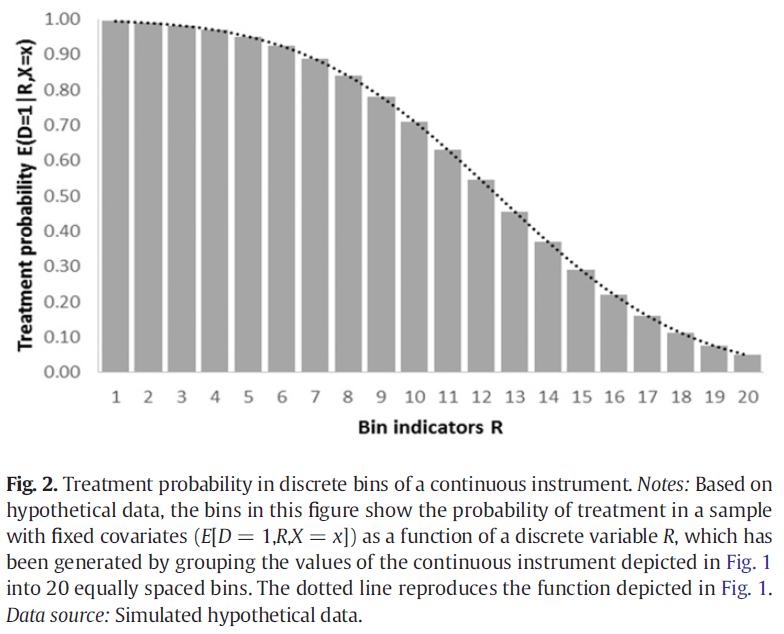
\includegraphics[width=.9\textwidth]{./resources/CornelissenBins}
  \end{center}  
\end{frame}

\begin{frame}
  \frametitle{Grouped IV averages relationship across bins}
  \begin{center}
    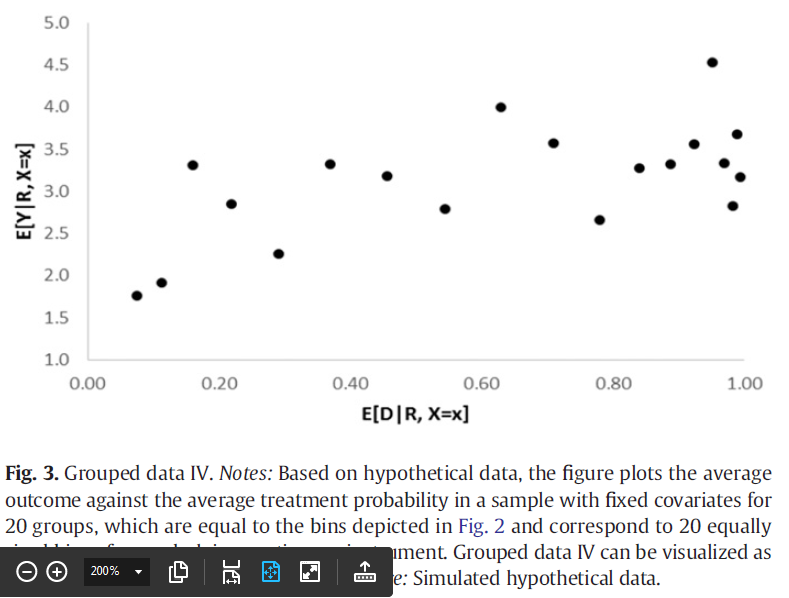
\includegraphics[width=.9\textwidth]{./resources/CornelissenGrouped}
  \end{center}  
\end{frame}

\begin{frame}
  \footnotesize
  \frametitle{How does this compare to IV?}
  \begin{itemize}
    \item 2SLS is going to fit a line through these heterogenous effects, and aggregate IV will be the slope. 
    \item MTE allows slope to vary across very fine bins 
    \item Looking at the Wald formula, can see that MTE for a given $u_s$ is the limit of LATE as $P(z') \rightarrow P(z)$ 
    \item Thus the MTE is actually identified from local IV (LIV) using small departures from propensity score at $u_{s} = P(z)$
  \end{itemize}
\end{frame}

\begin{frame}
  \footnotesize
  \frametitle{How does this compare to IV?}
  \begin{itemize}
    \item 2SLS is going to fit a line through these heterogenous effects, and aggregate IV will be the slope. 
    \item MTE allows slope to vary across very fine bins 
    \item Looking at the Wald formula, can see that MTE for a given $u_s$ is the limit of LATE as $P(z') \rightarrow P(z)$ 
    \item Thus the MTE is actually identified from local IV (LIV) using small departures from propensity score at $u_{s} = P(z)$
  \end{itemize}
\end{frame}

\begin{frame}
  \frametitle{HV ECMA 2005 show everything is a weighted MTE}
  \begin{center}
    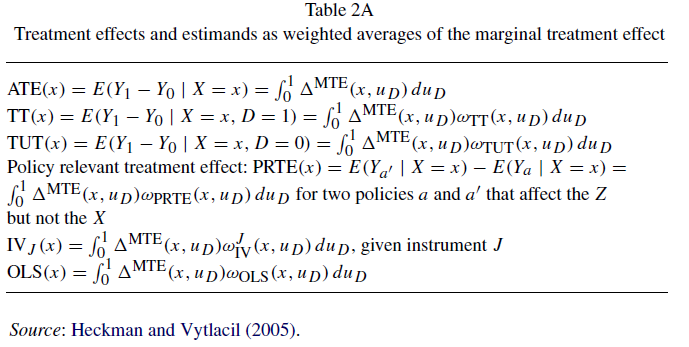
\includegraphics[width=\textwidth]{./resources/HVMTEmap}
  \end{center}  
\end{frame}

\begin{frame}
  \frametitle{HV ECMA 2005 show everything is a weighted MTE}
  \begin{center}
    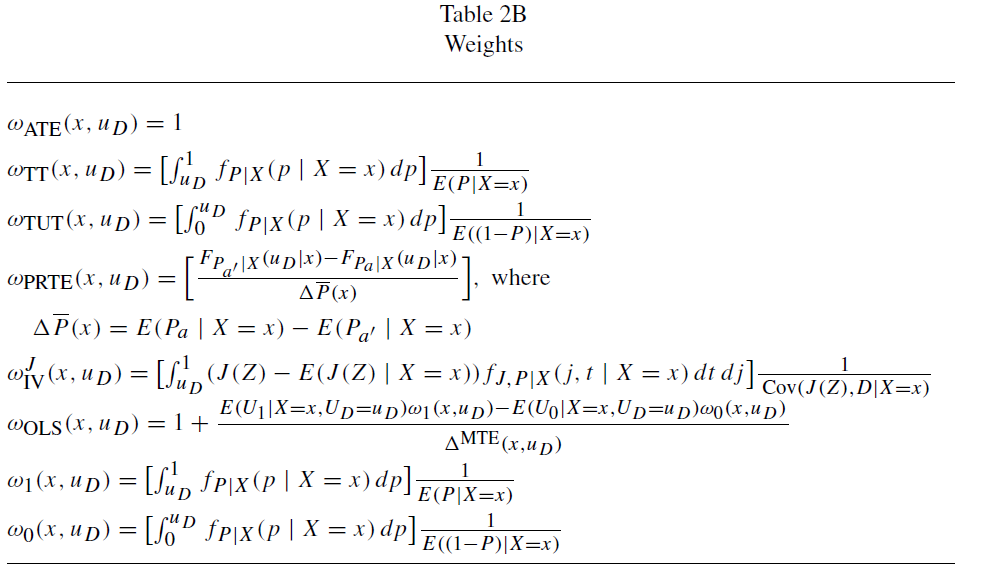
\includegraphics[width=\textwidth]{./resources/HVWeights}
  \end{center}  
\end{frame}

\begin{frame}
  \frametitle{Policy Relevant TE}
  \begin{center}
    \includegraphics[width=\textwidth]{./resources/HVPRTE}
  \end{center}  
\end{frame}

\begin{frame}
  \frametitle{HV Roy Example}
  \begin{center}
    \includegraphics[width=.9\textwidth]{./resources/HVRoyTEs}
  \end{center}  
\end{frame}

\begin{frame}
  \frametitle{HV Roy Example}
  \vspace{-10pt}
  \begin{center}
    \includegraphics[width=\textwidth]{./resources/HVOLSIVexample}
  \end{center}  
\end{frame}

\begin{frame}
  \frametitle{\cite{carneiro2011estimating}}
  \begin{itemize}
  \item Estimate returns to college (including heterogeneity of returns). $T_i =1$ if ever attended college. 
  \item NLSY 1979
  \item $Y = \log(wage)$ in 1991
  \item Covariates $X$: Experience (years), Ability (AFQT Score), Mother's Education, Cohort Dummies, State Unemployment, MSA level average wage.
  \item Instruments $Z$: 
  \begin{itemize}
    \item Cost shifters: College in MSA ; In state cost
    \item Opportunity cost: average earnings in MSA and avg unemployment (at 17).
  \end{itemize}

  \end{itemize}
\end{frame}

\begin{frame}
  \frametitle{Propensity estimate: Logit}
  \vspace{-10pt}
  \begin{center}
    \includegraphics[width=.9\textwidth]{./resources/CarnieroFirstStage}
  \end{center}  
\end{frame}

\begin{frame}
  \frametitle{Carneiro, Heckman and Vytlacil}
  \begin{center}
  \includegraphics[width=4in]{./resources/chv_tab4}
  \end{center}
\end{frame}

\begin{frame}
\frametitle{CHV Normal Selection Model}
\vspace{-10pt}
\begin{center}
\includegraphics[width= \textwidth]{./resources/chv_fig1}
\end{center}
\end{frame}


\begin{frame}
\frametitle{Carneiro, Heckman and Vytlacil}
\begin{center}
\includegraphics[width=4in]{./resources/chv_tab5}
\end{center}
\end{frame}

\begin{frame}
  \frametitle{CHV Don't Have Full Support}
  \vspace{-10pt}
  \begin{center}
  \includegraphics[width= \textwidth]{./resources/CarnieroSupport}
  \end{center}
\end{frame}
  
\begin{frame}
  \frametitle{CHV Local IV MTE}
\vspace{-20pt}
\begin{center}
\includegraphics[width= 1.05\textwidth]{./resources/chv_fig4}
\end{center}
\end{frame}

\begin{frame}
  \frametitle{CHV Local IV MTE}
  \begin{center}
  \includegraphics[width=4in]{./resources/chv_fig6}
  \end{center}
\end{frame}
  

\begin{frame}
  \frametitle{What does this tell us?}
  \begin{itemize}
  \item Huge difference in returns
  \item Negative selection: people with lowest resistance have returns of 40 percent. For those with highest restistance its a 20 percent loss. 
  \item Suggests people know something we don't when they opt out of college.  
  \item Obviously ATE would be very misleading here. 
  
  \end{itemize}
\end{frame}

\begin{frame}
  \frametitle{Selection doesn't have to be positive}
  Cornellissen 2016: universal pre-K program in Germany. 
  \begin{center}
    \includegraphics[width= .9\textwidth]{./resources/CornelissenNegative}
   \end{center}
    
\end{frame}

\begin{frame}
  \frametitle{Summary: Margins Matter}
  \begin{center}
    \includegraphics[width= \textwidth]{./resources/CornelissenSummary}
   \end{center}
\end{frame}

\begin{frame}
\frametitle{Diversion Example}
I have done some work trying to bring these methods into merger analysis.
\begin{itemize}
\item Key quantity: \alert{Diversion Ratio} as I raise my price, how much do people switch to a particular competitor's product
\begin{eqnarray*}
D_{jk}(p_j,p_{-j}) = \left| \frac{\partial q_k}{\partial p_j}(p_j,p_{-j}) /  \frac{\partial q_j}{\partial p_j}(p_j,p_{-j}) \right|
\end{eqnarray*}
\item We hold $p_{-j}$ fixed and trace out $D_{jk}(p_j)$.
\item The \alert{treatment} is leaving good $j$.
\item The $Y_i$ is increased sales of good $k$.
\item The $Z_i$ is the price of good $j$.
\item The key is that all changes in sales of $k$ come through people leaving good $j$ (no direct effects).
\end{itemize}
\end{frame}

\begin{frame}
\frametitle{Diversion for Prius (FAKE!)}
\begin{center}
\includegraphics[width=4in]{./resources/sillydiversion.pdf}
\end{center}
\end{frame}

\begin{frame}
\frametitle{Diversion Example}
\begin{eqnarray*}
\label{weighteddiversion}
\widehat{D_{jk}^{LATE} }&=& \frac{1}{\Delta q_j} \int_{p_j^{0}}^{p_j^{0}+\Delta p_j} \underbrace{\frac{\partial q_k(p_j,p^{0}_{-j})}{\partial q_j}}_{\equiv D_{jk}(p_j,p^{0}_{-j})} \left| \frac{\partial q_j(p_j,p^{0}_{-j})}{\partial p_j} \right|\, dp_j
\end{eqnarray*}
\begin{itemize}
\item $D_{jk}(p_j,p^{0}_{-j})$ is the MTE.
\item Weights $w(p_j) = \frac{1}{\Delta q_j} \frac{\partial q_j(p_j,p^{0}_{-j})}{\partial p_j}$ correspond to the lost sales of $j$ at a particular $p_j$ as a fraction of all lost sales.
\item When is $LATE \approx ATE$? 
\begin{itemize}
\item Demand for Prius is steep: everyone leaves right away
\item $D_{j,k}(p_j)$ is relatively flat.
\item We might want to think about raising the price to choke price (or eliminating the product from the consumers choice set) same as treating everyone!
\end{itemize}
\end{itemize}
\end{frame}

%%%%%%%%%%%%%%%%%%%%%%%%%%%%%%%%%%%%%%%%%%%%%%%%%%%%%%%%%%%%%%%%%%%%%
\begin{frame}[allowframebreaks]
  \bibliographystyle{jpe}
  \bibliography{../empirical-methods}
\end{frame}

%%%%%%%%%%%%%%%%%%%%%%%%%%%%%%%%%%%%%%%%%%%%%%%%%%%%%%%%%%%%%%%%%%%%%%
\section*{Backup}

\end{document}
